% Basic Category Theory
% Tom Leinster <Tom.Leinster@ed.ac.uk>
% 
% Copyright (c) Tom Leinster 2014-2016
% 
% Chapter 5: Limits
% 

\chapter{Limits}
\label{ch:lims}


Limits, and the dual concept, colimits, provide our third approach to the
idea of universal property.  

Adjointness is about the relationships \emph{between} categories.
Representability is a property of \emph{set-valued} functors.  Limits are
about what goes on \emph{inside} a category.

The concept of limit unifies many familiar constructions in mathematics.
Whenever you meet a method for taking some objects and maps in a category
and constructing a new object out of them, there is a good chance that you
are looking at either a limit or a colimit.  For instance, in group theory,
we can take a homomorphism between two groups and form its kernel, which
is a new group.  This construction is an example of a limit in the category
of groups.  Or, we might take two natural numbers and form their lowest
common multiple.  This is an example of a colimit in the poset of natural
numbers, ordered by divisibility.



\section{Limits: definition and examples}
\label{sec:lims-basics}


The definition of limit is very general.  We build up to it by first
examining some particularly useful types of limit: products, equalizers,
and pullbacks.


\minihead{Products}


Let $X$ and $Y$ be sets.  The familiar cartesian product%
%
\index{set!category of sets!products in}
%
$X \times Y$ is characterized by the property that an element of $X \times
Y$ is an element of $X$ together with an element of $Y$.  Since elements
are just maps from $1$, this says that a map $1 \to X \times Y$ amounts to
a map $1 \to X$ together with a map $1 \to Y$.

A little thought reveals that the same is true when $1$ is replaced
throughout by any set $A$ whatsoever.  (In other words, a generalized
element of $X \times Y$ of shape $A$ amounts to a generalized element of
$X$ of shape $A$ together with a generalized element of $Y$ of shape $A$.)
The bijection between
\[
\text{maps } A \to X \times Y
\]
and
\[
\text{pairs of maps } (A \to X,\ A \to Y)
\]
is given by composing with the projection maps
\[
\begin{array}{ccccc}
X       &\otby{p_1}     &X \times Y     &\toby{p_2}     &Y      \\
x       &\mapsfrom      &(x, y)         &\mapsto        &y.
\end{array}
\]
This suggests the following definition.

\begin{defn}    
\label{defn:bin-prod}
Let $\cat{A}$ be a category and $X, Y \in \cat{A}$.  A \demph{product}%
%
\index{product}
%
of $X$ and $Y$ consists of an object $P$ and maps
\[
\xymatrix{
        &P \ar[ld]_{p_1} \ar[rd]^{p_2}  &       \\
X       &                               &Y
}
\]
with the property that for all objects and maps
% 
\begin{equation}        
\label{eq:bin-prod-cone}
\begin{array}{c}
\xymatrix{
        &A \ar[ld]_{f_1} \ar[rd]^{f_2}  &       \\
X       &                               &Y
}
\end{array}
\end{equation}
% 
in $\cat{A}$, there exists a unique map $\bar{f}\from A \to P$ such that 
% 
\begin{equation}        
\label{eq:bin-prod-lim}
\begin{array}{c}
\xymatrix{
        &A \ar[ldd]_{f_1} \ar@{.>}[d]|{\bar{f}\vphantom{\bar{\bar{f}}}} 
\ar[rdd]^{f_2}&       \\
        &P \ar[ld]^{p_1} \ar[rd]_{p_2}                  &       \\
X       &                                               &Y
}
\end{array}
\end{equation}
% 
commutes.  The maps $p_1$ and $p_2$ are called the \demph{projections}.%
%
\index{projection}
%
\end{defn}

\begin{remarks} 
\label{rmks:prod}
\begin{enumerate}[(b)]
\item   
\label{rmks:prod:exist}
Products do not always exist.  For example, if $\cat{A}$ is the discrete
two-object category
\[
\fbox{$X\bullet$ \hspace*{2em} $\bullet Y$}
\]
then $X$ and $Y$ do not have a product.  But when objects $X$ and $Y$ of a
category do have a product, it is unique%
%
\index{product!uniqueness of} 
%
up to isomorphism.  (This can be proved directly, much as in
Lemma~\ref{lemma:init-unique}.  It also follows from
Corollary~\ref{cor:lims-unique}.)  This justifies talking about \emph{the}
product of $X$ and $Y$.

\item 
Strictly speaking, the product consists of the object $P$ \emph{together
  with} the projections $p_1$ and $p_2$.  But informally,%
%
\index{product!informal usage}
%
we often refer to $P$ alone as the product of $X$ and $Y$.  We write $P$ as
$X \times Y$.%
%
\ntn{prod-gen}
%
\end{enumerate}
\end{remarks}


\begin{example}
\label{eg:sets}
Any two sets $X$ and $Y$ have a product%
%
\index{set!category of sets!products in}
%
in $\Set$.  It is the usual cartesian product $X \times Y$, equipped with
the usual projection maps $p_1$ and $p_2$.

Let us check that this really is a product in the sense of
Definition~\ref{defn:bin-prod}.  Take sets and functions as in
diagram~\eqref{eq:bin-prod-cone}.  Define $\bar{f}\from A \to X \times Y$
by $\bar{f}(a) = (f_1(a), f_2(a))$.  Then $p_i \of \bar{f} = f_i$ for $i =
1, 2$; that is, diagram~\eqref{eq:bin-prod-lim} commutes with $P = X \times
Y$.  Moreover, this is the \emph{only} map making
diagram~\eqref{eq:bin-prod-lim} commute.  For suppose that $\hat{f}\from A
\to X \times Y$, in place of $\bar{f}$, also makes~\eqref{eq:bin-prod-lim}
commute.  Let $a \in A$, and write $\hat{f}(a)$ as $(x, y)$.  Then
\[
f_1(a) = p_1(\hat{f}(a)) = p_1(x, y) = x,
\]
and similarly, $f_2(a) = y$.  Hence $\hat{f}(a) = (f_1(a), f_2(a)) =
\bar{f}(a)$ for all $a \in A$, giving $\hat{f} = \bar{f}$, as required.
\end{example}

In general, in any category, the map $\bar{f}$ of
diagram~\eqref{eq:bin-prod-lim} is usually written as $(f_1, f_2)$.

\begin{example}
\label{eg:prod-spaces}
In the category of topological spaces, any two objects $X$ and $Y$ have a
product.%
%
\index{topological space!category of topological spaces!products in}
%
It is the set $X \times Y$ equipped with the product topology and the
standard projection maps.  The product topology is deliberately designed so
that a function
\[
\begin{array}{ccc}
A       &\to            &X \times Y     \\
t       &\mapsto        &(x(t), y(t))
\end{array}
\]
is continuous if and only if it is continuous in each coordinate (that is to
say, both functions
\[
t \mapsto x(t),
\qquad
t \mapsto y(t)
\]
are continuous).  This holds for any space $A$, but the idea is perhaps at
its most intuitively appealing when $A = \reals$ and we think of $t$ as a
time parameter.

A closely related statement is that the product topology is the smallest
topology on $X \times Y$ for which the projections are continuous.  Here
`smallest' means that for any other topology $\mathcal{T}$ on $X \times Y$
such that $p_1$ and $p_2$ are continuous, every subset of $X \times Y$ open
in the product topology is also open in $\mathcal{T}$.  Thus, to define the
product topology, we declare just enough sets to be open that the
projections are continuous.
\end{example}

\begin{example}
\label{eg:prod-vs}
Now let $X$ and $Y$ be vector spaces.  We can form their direct sum,%
%
\index{vector space!direct sum of vector spaces}%
\index{vector space!category of vector spaces!products in}
%
$X \oplus Y$,%
%
\ntn{direct-sum}
%
whose elements can be written as either $(x, y)$ or $x + y$ (with $x \in
X$ and $y \in Y$), according to taste.  There are linear projection maps
\[
\xymatrix{
        &X \oplus Y \ar[ld]_{p_1} \ar[rd]^{p_2}     &       \\
X       &                                               &Y
}
% 
\qquad
% 
\xymatrix{
        &(x, y) \ar@{|->}[ld] \ar@{|->}[rd]     &       \\
x       &                                       &y.
}
\]
It can be shown that $X \oplus Y$, together with $p_1$ and $p_2$, is the
product of $X$ and $Y$ in the category of vector spaces
(Exercise~\ref{ex:prod-vs}).
\end{example}

\begin{examples}[Elements of ordered sets]     
\label{eg:prod-order}
%
\index{ordered set!product in|(}
%
\begin{enumerate}[(b)]
\item 
Let $x, y \in \reals$.  Their minimum $\min\{x, y\}$ satisfies
\[
\min\{x, y\} \leq x,
\qquad
\min\{x, y\} \leq y
%
\index{minimum}
%
\]
and has the further property that whenever $a \in \reals$ with
\[
a \leq x,
\qquad 
a \leq y,
\]
we have $a \leq \min\{x, y\}$.  This means exactly that when the poset
$(\reals, \mathord{\leq})$ is viewed as a category, the product of $x, y
\in \reals$ is $\min\{x, y\}$.  The definition of product simplifies when
interpreted in a poset, since all diagrams commute.

\item 
Fix a set $S$.  Let $X, Y \in \pset(S)$.%
%
\index{power!set}
%
Then $X \cap Y$%
%
\index{intersection}
%
satisfies
\[
X \cap Y \sub X,
\qquad
X \cap Y \sub Y
\]
and has the further property that whenever $A \in \pset(S)$ with
\[
A \sub X,
\qquad
A \sub Y,
\]
we have $A \sub X \cap Y$.  This means that $X \cap Y$ is the product of
$X$ and $Y$ in the poset $(\pset(S), \mathord{\sub})$ regarded as a
category.

\item 
Let $x, y \in \nat$.  Their greatest%
%
\index{greatest common divisor}
%
common divisor $\gcd(x, y)$ satisfies
\[
\gcd(x, y) \divides x,
\qquad
\gcd(x, y) \divides y
\]
(it's a common divisor!)\ and has the further property that whenever $a \in
\nat$ with
\[
a \divides x,
\qquad
a \divides y,
\]
we have $a \divides \gcd(x, y)$.  This means that $\gcd(x, y)$ is the
product of $x$ and $y$ in the poset $(\nat, \mathord{\mid})$ regarded as a
category.
\end{enumerate}

Generally, let $(A, \mathord{\leq})$ be a poset and $x, y \in A$.  A
\demph{lower%
%
\index{lower bound}
%
bound} for $x$ and $y$ is an element $a \in A$ such that $a
\leq x$ and $a \leq y$.  A \demph{greatest%
%
\index{greatest lower bound}
%
lower bound} or \demph{meet}%
%
\index{meet}
%
of $x$ and $y$ is a lower bound $z$ for $x$ and $y$ with the further
property that whenever $a$ is a lower bound for $x$ and $y$, we have $a
\leq z$.

When a poset is regarded as a category, meets are exactly products.  They do
not always exist, but when they do, they are unique.  The meet of $x$ and $y$
is usually written as $x \meet y$%
%
\ntn{meet}
%
rather than $x \times y$.  Thus, in the three examples above,
\[
x \meet y = \min\{x, y\},
\qquad
X \meet Y = X \cap Y,
\qquad
x \meet y = \gcd(x, y),
\]
the second example being the origin of the notation.%
%
\index{ordered set!product in|)}
%
\end{examples}

We have been discussing products $X \times Y$ of \emph{two} objects,
so-called \demph{binary%
%
\index{product!binary}
%
products}.  But there is no reason to stick to two.  We can just as well
talk about products $X \times Y \times Z$ of three objects, or of
infinitely many objects.  The definition changes in the most obvious way:

\begin{defn}    
\label{defn:gen-prod}
Let $\cat{A}$ be a category, $I$ a set, and $(X_i)_{i \in I}$ a family of
objects of $\cat{A}$.  A \demph{product}%
%
\index{product}
%
of $(X_i)_{i \in I}$ consists of an object $P$ and a family of maps
\[
\Bigl(P \toby{p_i} X_i\Bigr)_{i \in I}
\]
with the property that for all objects $A$ and families of maps
% 
\begin{equation}        
\label{eq:gen-prod-cone}
\Bigl(A \toby{f_i} X_i\Bigr)_{i \in I}
\end{equation}
% 
there exists a unique map $\bar{f}\from A \to P$ such that $p_i \of \bar{f} =
f_i$ for all $i \in I$.
\end{defn}

Remarks~\ref{rmks:prod} apply equally to this definition.  When the product
$P$ exists, we write $P$ as $\prod_{i \in I} X_i$%
%
\ntn{prod-fam-gen}
%
and the map $\bar{f}$ as $(f_i)_{i \in I}$.%
%
\ntn{map-to-prod}
%
We call the maps $f_i$ the \demph{components}%
%
\index{component!map into product@of map into product}
%
of the map $(f_i)_{i \in I}$.  Taking $I$ to be a two-element set, we
recover the special case of binary products.

\begin{example}        
In ordered sets, the extension from binary to arbitrary products works in
the obvious way: given an ordered set $(A, \mathord{\leq})$, a
\demph{lower%
%
\index{lower bound}
%
bound} for a family $(x_i)_{i \in I}$ of elements is an element $a \in A$
such that $a \leq x_i$ for all $i$, and a \demph{greatest%
%
\index{greatest lower bound}
%
lower bound} or \demph{meet}%
%
\index{meet}
%
of the family is a lower bound greater than any other, written as $\Meet_{i
\in I} x_i$.%
%
\ntn{Meet}
%
These are the products in $(A, \mathord{\leq})$.

For example, in $\reals$ with its usual ordering, the meet of a family
$(x_i)_{i \in I}$ is $\inf\{x_i \such i \in I\}$%
%
\index{infimum}
%
(and one exists if and only if the other does).
\end{example}

\begin{example}
\label{eg:arb-prods-terminal}
What happens to the definition of product when the indexing set $I$ is
empty?%
%
\index{product!empty}
%
Let $\cat{A}$ be a category.  In general, an $I$-indexed family
$(X_i)_{i \in I}$ of objects of $\cat{A}$ is a function $I \to
\ob(\cat{A})$.  When $I$ is empty, there is exactly one such function.  In
other words, there is exactly one family $(X_i)_{i \in \emptyset}$, the
\demph{empty%
%
\index{empty family}%
\index{family!empty}
%
family}.  Similarly, when $I$ is empty, there is exactly one
family~\eqref{eq:gen-prod-cone} for any given object $A$.

A product of the empty family therefore consists of an object $P$ of $\cat{A}$
such that for each object $A$ of $\cat{A}$, there exists a unique map
$\bar{f}\from A \to P$.  (The condition `$p_i \of \bar{f} = f_i$ for all $i
\in I$' holds trivially.)  In other words, a product of the empty family is
exactly a terminal%
%
\index{object!terminal}
%
object.

We have been writing $1$%
%
\ntn{terminal}
%
for terminal objects, which was justified by the fact that in categories
such as $\Set$, $\Tp$, $\Ring$ and $\Grp$, the terminal object has one%
%
\index{set!one-element}
%
element.  But we have just seen that the terminal object is the product of
no things, which in the context of elementary arithmetic%
%
\index{arithmetic}
% 
is the number $1$.  This is a second, related, reason for the notation.
\end{example}

\begin{example}
Take an object $X$ of a category $\cat{A}$, and a set $I$.  There is a
constant family $(X)_{i \in I}$.  Its product $\prod_{i \in I} X$, if it
exists, is written as $X^I$%
%
\ntn{power-of-obj}
%
and called a \demph{power}%
%
\index{power}
%
of $X$.  

We met powers in $\Set$ in Section~\ref{sec:Set-properties}.  When $X$ is a
set, $X^I$ is the set of functions from $I$ to $X$, also written as
$\Set(I, X)$.
\end{example}


\minihead{Equalizers}


To define our second type of limit, we need a preliminary piece of
terminology: a \demph{fork}%
%
\index{fork}
%
in a category consists of objects and maps
% 
\begin{equation}        
\label{eq:fork}
\xymatrix{
A \ar[r]^f   &
X \ar@<.5ex>[r]^s \ar@<-.5ex>[r]_t    &
Y
}
\end{equation}
% 
such that $sf = tf$.

\begin{defn}    
\label{defn:equalizer}
Let $\cat{A}$ be a category and let $\parpairi{X}{Y}{s}{t}$ be objects and
maps in $\cat{A}$.  An \demph{equalizer}%
%
\index{equalizer}
%
of $s$ and $t$ is an object $E$ together with a map $E \toby{i} X$ such
that
\[
\xymatrix{
E \ar[r]^i   &
X \ar@<.5ex>[r]^s \ar@<-.5ex>[r]_t    &
Y
}
\]
is a fork, and with the property that for any fork~\eqref{eq:fork},
there exists a unique map $\bar{f}\from A \to E$ such that
% 
\begin{equation}        
\label{eq:equalizer-whole}
\begin{array}{c}
\xymatrix{
A \ar@{.>}[d]_{\bar{f}} \ar[rd]^f    &       \\
E \ar[r]_i                      &X
}
\end{array}
\end{equation}
% 
commutes.
\end{defn}

Remarks~\ref{rmks:prod} on products apply to equalizers too.

\begin{example}
\label{eg:equalizers-Set}
We have already met equalizers%
%
\index{set!category of sets!equalizers in}%
\index{equalizer!sets@of sets}
%
in $\Set$ (Section~\ref{sec:Set-properties}).  They really are equalizers
in the sense of Definition~\ref{defn:equalizer}.  Indeed, take sets and
functions $\parpairi{X}{Y}{s}{t}$\!, write
\[
E = \{ x \in X \such s(x) = t(x) \},
\]
and write $i\from E \to X$ for the inclusion.  Then $s i = t i$, so we have
a fork, and one can check that it is universal among all forks on $s$ and
$t$.

An equalizer describes the set of solutions of a single equation, but by
combining equalizers with products, we can also describe the solution-set
of any system of simultaneous%
%
\index{simultaneous equations}
%
equations.  Take a set $\Lambda$ and a family 
\[
\biggl( 
\parpair{X}{Y_\lambda}{s_\lambda}{t_\lambda} 
\biggr)_{\lambda \in \Lambda} 
\]
of pairs of maps in $\Set$.  Then the solution-set
\[
\{ 
x \in X 
\such
s_\lambda(x) = t_\lambda(x) \text{ for all } \lambda \in \Lambda 
\} 
\]
is the equalizer of the functions
\[
\xymatrix@C+1em{
X
\ar@<.5ex>[r]^-{(s_\lambda)_{\lambda \in \Lambda}}
\ar@<-.5ex>[r]_-{(t_\lambda)_{\lambda \in \Lambda}}        &
\raisebox{-4.2ex}{$\displaystyle \prod_{\lambda \in \Lambda} Y_\lambda$}
}
\]
(using the notation introduced after Definition~\ref{defn:gen-prod}).  To
see this, observe that for $x \in X$,
% 
\begin{align*}
(s_\lambda)_{\lambda \in \Lambda}(x) =
(t_\lambda)_{\lambda \in \Lambda}(x) &
\iff
\bigl(s_\lambda(x)\bigr)_{\lambda \in \Lambda} = 
\bigl(t_\lambda(x)\bigr)_{\lambda \in \Lambda}  \\
&
\iff
s_\lambda(x) = t_\lambda(x) \text{ for all } \lambda \in \Lambda,
\end{align*}
% 
as required.
\end{example}

\begin{example}
Take continuous maps $\parpairi{X}{Y}{s}{t}$ between topological\linebreak
spaces.  We can form their equalizer%
%
\index{topological space!category of topological spaces!equalizers in}
%
$E$ in the category of sets, with inclusion map $i\from E \to X$, say.
Since $E$ is a subset of the space $X$, it acquires the subspace%
%
\index{topological space!subspace of}
%
topology from $X$, and $i$ is then continuous.  This space $E$, together
with $i$, is the equalizer of $s$ and $t$.

Showing this amounts to showing that for any fork~\eqref{eq:fork} in
$\Tp$, the induced function $\bar{f}$ is continuous.  This follows from
the definition of the subspace topology, which is the smallest topology
such that the inclusion map is continuous.  Compare the remarks on products
in Example~\ref{eg:prod-spaces}.
\end{example}

\begin{example}
Let $\theta\from G \to H$ be a homomorphism of groups.  As in
Example~\ref{eg:univ-kernel}, the homomorphism $\theta$ gives rise to a fork
\[
\xymatrix{
\ker\theta\      \ar@{^{(}->}[r]^-\iota   &
G \ar@<.5ex>[r]^\theta \ar@<-.5ex>[r]_\epsln    &
H
}
%
\index{kernel}
%
\]
where $\iota$ is the inclusion and $\epsln$ is the trivial homomorphism.
This is an equalizer%
%
\index{group!category of groups!equalizers in}
%
in $\Grp$.  Showing this amounts to showing that the map that we have been
calling $\bar{f}$ is a homomorphism, which is left to the reader.

Thus, kernels are a special case of equalizers.
\end{example}

\begin{example} 
\label{eg:eq-vect}
Let $\parpairi{V}{W}{s}{t}$ be linear maps between vector spaces.\linebreak  
There is a linear map $t - s \from V \to W$, and the equalizer%
%
\index{vector space!category of vector spaces!equalizers in}
%
of $s$ and $t$ in the category of vector spaces is the space $\ker(t - s)$%
%
\index{kernel}
%
together with the inclusion map $\ker(t - s) \incl V$.
\end{example}


\minihead{Pullbacks}


We explore one more type of limit before formulating the general
definition. 

\begin{defn}    
\label{defn:pb}
Let $\cat{A}$ be a category, and take objects and maps
% 
\begin{equation}        
\label{eq:pb-corner}
\begin{array}{c}
\xymatrix{
                &Y \ar[d]^t     \\
X \ar[r]_s      &Z
}
\end{array}
\end{equation}
% 
in $\cat{A}$.  A \demph{pullback}%
%
\index{pullback}
%
of this diagram is an object $P \in \cat{A}$ together with maps $p_1\from P
\to X$ and $p_2\from P \to Y$ such that
% 
\begin{equation}        
\label{eq:pb}
\begin{array}{c}
\xymatrix{
P \ar[r]^{p_2} \ar[d]_{p_1}     &
Y \ar[d]^t      \\
X \ar[r]_s      &
Z
}
\end{array}
\end{equation}
% 
commutes, and with the property that for any commutative square
% 
\begin{equation}        
\label{eq:pb-cone}
\begin{array}{c}
\xymatrix{
A \ar[r]^{f_2} \ar[d]_{f_1}     &
Y \ar[d]^t      \\
X \ar[r]_s      &
Z
}
\end{array}
\end{equation}
% 
in $\cat{A}$, there is a unique map $\bar{f}\from A \to P$ such that
% 
\begin{equation}        
\label{eq:pb-whole}
\begin{array}{c}
\xymatrix{
A \ar@/^/[rrd]^{f_2} \ar@{.>}[rd]|{\bar{f}} \ar@/_/[rdd]_{f_1}&       
        &       \\
        &
P \ar[r]^{p_2} \ar[d]_{p_1}     &
Y \ar[d]^t      \\
        &
X \ar[r]_s      &Z
}
\end{array}
\end{equation}
% 
commutes.  (For~\eqref{eq:pb-whole} to commute means only that $p_1 \bar{f}
= f_1$ and $p_2 \bar{f} = f_2$, since the commutativity of the square is
already given.)
\end{defn}

Again, Remarks~\ref{rmks:prod} apply.  

We call~\eqref{eq:pb} a \demph{pullback%
%
\index{pullback!square}
%
square}.  Another name for pullback is \demph{fibred%
%
\index{fibred product}
%
product}.  This name is partially explained by the following fact: when $Z$
is a terminal object (and $s$ and $t$ are the only maps they can possibly
be), a pullback of the diagram~\eqref{eq:pb-corner} is simply a product%
%
\index{product!pullback@as pullback}
%
of $X$ and $Y$.

\begin{examples}[Pullbacks in $\Set$]
\label{egs:pb-sets}
The pullback of a diagram~\eqref{eq:pb-corner} in $\Set$ is
\[
P = \{ (x, y) \in X \times Y \such s(x) = t(y) \}
\]
with projections $p_1$ and $p_2$ given by $p_1(x, y) = x$ and $p_2(x, y) =
y$. 

Although you might not be familiar with general pullbacks in $\Set$, there are
at least two instances that you are likely to have met.
% 
\begin{enumerate}[(b)]
\item   
\label{eg:pb-sets-inv}
A basic construction with sets and functions is the formation of inverse%
%
\index{inverse!image!pullback@as pullback}
%
images.  They are an instance of pullbacks.  Indeed, given a function
$f\from X \to Y$ and a subset $Y' \sub Y$, we obtain a new set, the inverse
image
\[
f^{-1}Y' 
=
\{ x \in X \such f(x) \in Y' \} \sub X,
\]
and a new function,
\[
\begin{array}{cccc}
f'\from         &f^{-1} Y'      &\to            &Y'     \\
                &x              &\mapsto        &f(x).
\end{array}
\]
We also have the inclusion functions $j\from Y' \incl Y$ and $i\from f^{-1}Y'
\incl X$.  Putting everything together gives a commutative square
% 
\begin{equation}        
\label{eq:pb-inv}
\begin{array}{c}
\xymatrix@M+.5ex{
f^{-1}Y' \ar[r]^{f'} \ar@{^{(}->}[d]_i &
Y' \ar@{^{(}->}[d]^j   \\
X \ar[r]_f      &
Y.
}
\end{array}
\end{equation}
% 
The data we started with was the lower-right part of this square ($X$, $Y$,
$Y'$, $f$ and $j$), and from it we constructed the rest of the square
($f^{-1} Y'$, $f'$ and $i$).

The square~\eqref{eq:pb-inv} is a pullback.  Let us verify this in detail.
Take any commutative square
\[
\xymatrix@M+.5ex{
A \ar[r]^h \ar[d]_g     &
Y' \ar@{^{(}->}[d]^j   \\
X \ar[r]_f      &
Y.
}
\]
We must show that there is a unique map $k\from A \to f^{-1}Y'$ such that
\[
\xymatrix@M+.5ex{
A \ar@/^/[rrd]^h \ar@{.>}[rd]|k \ar@/_/[rdd]_g  &       &       \\
                                        &
f^{-1}Y' \ar[r]_-{f'} \ar@{^{(}->}[d]^-i       &
Y' \ar@{^{(}->}[d]^j   \\
        &
X \ar[r]_f      &Y
}
\]
commutes.  For uniqueness, let $k$ be a map making the diagram commute.
Then for all $a \in A$, we have $i(k(a)) = g(a)$, that is, $k(a) = g(a)$,
and this determines $k$ uniquely.  For existence, first note that for all
$a \in A$ we have $f(g(a)) = j(h(a)) \in Y'$, so $g(a) \in f^{-1}Y'$.
Hence we may define $k\from A \to f^{-1} Y'$ by $k(a) = g(a)$ for all $a
\in A$.  Then for all $a \in A$, we have $i(k(a)) = k(a) = g(a)$ and
\[
f'(k(a)) = f(k(a)) = f(g(a)) = j(h(a)) = h(a).
\]
Hence $i \of k = g$ and $f' \of k = h$, as required.

\item 
Intersection%
%
\index{intersection!pullback@as pullback}
%
of subsets provides another example of pullbacks.  Indeed, let $X$ and $Y$
be subsets of a set $Z$.  Then
\[
\xymatrix@M+.5ex{
X \cap Y \ar@{^{(}->}[r] \ar@{^{(}->}[d]        &
Y \ar@{^{(}->}[d]    \\
X \ar@{^{(}->}[r]       &
Z
}
\]
% 
is a pullback square, where all the arrows are inclusions of subsets.  

In fact, this is a special case of~\bref{eg:pb-sets-inv}, since $X \cap Y$ is
the inverse image of $Y \sub Z$ under the inclusion map $X \incl Z$.
\end{enumerate}
\end{examples}

In the situation of Example~\ref{egs:pb-sets}\bref{eg:pb-sets-inv}, where we
have a map $f\from X \to Y$ and a subset $Y'$ of $Y$, people sometimes say
that $f^{-1}Y'$ is obtained by `pulling $Y'$ back' along $f$: hence the name. 

\minihead{The definition of limit}

We have now looked at three constructions: products, equalizers and
pullbacks.  They clearly have something in common.  Each starts with some
objects and (in the case of equalizers and pullbacks) some maps between
them.  In each, we aim to construct a new object together with some maps
from it to the original objects, with a universal property.

Let us analyse this more closely.  What is the starting data in each
construction?  For (binary) products, it is a pair of objects
% 
\begin{equation}        
\label{eq:prod-data}
X \hspace*{3em} Y.
\end{equation}
% 
For equalizers, it is a diagram 
% 
\begin{equation}        
\label{eq:eq-data}
\parpair{X}{Y.}{s}{t}
\end{equation}
% 
For pullbacks, it is a diagram
% 
\begin{equation}        
\label{eq:pb-data}
\begin{array}{c}
\xymatrix{
                &Y \ar[d]^t     \\
X \ar[r]_s      &Z.
}
\end{array}
\end{equation}

In Definition~\ref{defn:gen-elt}, we met the notion of generalized%
%
\index{element!generalized}
%
element, and we saw there that the `figures' in a geometric object can often
be described by maps into it.  For instance, a curve in a topological space
$A$ can be thought of as a map $\reals \to A$.  Similarly, an object of a
category $\cat{A}$ amounts to a functor $D\from \One \to \cat{A}$; think of
$\One = \fbox{$\bullet$}$ as an unlabelled object and $D$ as labelling it
with the name of an object of $\cat{A}$.  And similarly again, a map in a
category $\cat{A}$ is a functor $\Two \to \cat{A}$, where $\Two =
\fbox{$\bullet \to \bullet$}$.%
%
\ntn{Two}
%
(Here $\Two$ is the category with two objects, say $0$ and $1$, with one
map $0 \to 1$, and with no other maps except for identities.)  Finally, if
we take $\scat{I}$ to be one of the categories
% 
\begin{equation}        
\label{eq:lim-shapes}
\scat{T} = 
\fbox{$\bullet \hspace*{2.5em} \bullet$}\ ,
% 
\quad
% 
\scat{E} = 
\fbox{$\parpair{\bullet}{\bullet}{}{}$}
% 
\quad
% 
\text{or}
% 
\quad
% 
\scat{P} =
\fbox{%
$\begin{array}{c}
\xymatrix{
                &\bullet \ar[d] \\
\bullet \ar[r]  &\bullet
}
\end{array}$}
\end{equation}
% 
then a functor $\scat{I} \to \cat{A}$ consists of data~\eqref{eq:prod-data},
\eqref{eq:eq-data} or~\eqref{eq:pb-data} in $\cat{A}$, respectively. 

We have just begun to use the convention that one typeface ($\scat{A}$,
$\scat{B}$,%
%
\ntn{small-cat-face}
%
$\scat{C}$, \ldots) denotes small%
%
\index{small}%
\index{category!small}
%
categories, and another ($\cat{A}$, $\cat{B}$,%
%
\ntn{arb-cat-face}
%
 $\cat{C}$, \ldots) denotes arbitrary categories.  Although not strictly
necessary, this convention is helpful, since small categories and arbitrary
categories often play different roles in the theory.

\begin{defn}    
\label{defn:diagram}
Let $\cat{A}$ be a category and $\scat{I}$ a small category.  A functor
$\scat{I} \to \cat{A}$ is called a \demph{diagram}%
%
\index{diagram}
%
in $\cat{A}$ of \demph{shape}%
%
\index{shape!diagram@of diagram}
%
$\scat{I}$.
\end{defn}

So~\eqref{eq:prod-data}, \eqref{eq:eq-data} and~\eqref{eq:pb-data} are
diagrams of shape $\scat{T}$, $\scat{E}$ and $\scat{P}$.  

We already have the definitions of product of a diagram of shape
$\scat{T}$, equalizer of a diagram of shape $\scat{E}$, and pullback of a
diagram of shape $\scat{P}$.  We now unify them in the definition of limit
(Figure~\ref{fig:defn-limit}).

\begin{figure}
\centering
\setlength{\unitlength}{1em}
\begin{picture}(18.5,12)(1,-1.5)
\cell{0}{0}{bl}{%
\begin{array}{c}
\xymatrix@C=6em{
        &       &D(I)   \\
A \ar[rru]^{f_I} \ar@{.>}[r]|{\,\exists! \bar{f}\,} \ar[rrd]_{f_J}  &
L \ar[ru]_{p_I} \ar[rd]^{p_J}   &       \\
        &       &D(J)
}
\end{array}
}
\put(16,4.5){\oval(4.5,12)}
\cell{19}{-1}{c}{D}
\end{picture}
\caption{The definition of limit.}  
\label{fig:defn-limit}
\end{figure}

\begin{defn}    
\label{defn:lim}
Let $\cat{A}$ be a category, $\scat{I}$ a small category, and $D\from \scat{I}
\to \cat{A}$ a diagram in $\cat{A}$.  
%
\begin{enumerate}[(b)]
\item
A \demph{cone}%
%
\index{cone}
%
on $D$ is an object $A \in \cat{A}$ (the \demph{vertex}%
%
\index{vertex}
%
of the cone) together with a family
% 
\begin{equation}        
\label{eq:gen-cone}
\Bigl(
A \toby{f_I} D(I)
\Bigr)_{I \in \scat{I}}
\end{equation}
% 
of maps in $\cat{A}$ such that for all maps $I \toby{u} J$ in $\scat{I}$, the
triangle
\[
\xymatrix@R=1ex{
                                &D(I) \ar[dd]^{Du}      \\
A \ar[ru]^{f_I} \ar[rd]_{f_J}   &                       \\
                                &D(J)
}
\]
commutes.  (Here and later, we abbreviate $D(u)$ as $Du$.)  

\item
A \demph{limit}%
%
\index{limit}
%
of $D$ is a cone $\Bigl(L \toby{p_I} D(I)\Bigr)_{I \in \scat{I}}$ with the
property that for any cone~\eqref{eq:gen-cone} on $D$, there exists a
unique map $\bar{f}\from A \to L$%
%
\ntn{lim-bar}
%
such that $p_I \of \bar{f} = f_I$ for all $I \in \scat{I}$.  The maps $p_I$
are called the \demph{projections}%
%
\index{projection}
%
of the limit.
\end{enumerate}
\end{defn}

\begin{remarks} 
\label{rmks:defn-lim}
\begin{enumerate}[(b)]
\item	
\label{rmk:defn-lim-univ} 
Loosely, the universal property says that for any $A \in \cat{A}$, maps $A
\to L$ correspond one-to-one with cones on $D$ with vertex $A$.  (Any map
$g\from A \to L$ gives rise to a cone $\Bigl( A \toby{p_I g} D(I) \Bigr)_{I
  \in \scat{I}}$, and the definition of limit is that for each $A$, this
process is bijective.)  In Section~\ref{sec:lra}, we will use this thought
to rephrase the definition of limit in terms of representability.  From
this it will follow that limits are unique up to canonical isomorphism,
when they exist (Corollary~\ref{cor:lims-unique}).  Alternatively,
uniqueness can be proved by the usual kind of direct argument, as in
Lemma~\ref{lemma:init-unique}.

\item 
If $\Bigl( L \toby{p_I} D(I) \Bigr)_{I \in \scat{I}}$ is a limit of $D$, we
sometimes abuse language slightly by referring to $L$ (rather than the
whole cone) as the limit%
%
\index{limit!informal usage}
%
of $D$.  For emphasis, we sometimes call $\Bigl( L \toby{p_I} D(I)
\Bigr)_{I \in \scat{I}}$ a \demph{limit%
%
\index{limit!cone}%
\index{cone!limit}
%
cone}.  We write $L = \lt{\scat{I}} D$.%
%
\ntn{lim}
%
Remark~\bref{rmk:defn-lim-univ} can then be stated as:
% 
\begin{slogan}
A map into $\lt{\scat{I}} D$ is a cone on $D$.
\end{slogan}

\item   
\label{rmks:defn-lim:small}
By assuming from the outset that the shape category $\scat{I}$ is small, we
are restricting ourselves to what are officially called \demph{small%
%
\index{limit!small}%
\index{small}
%
limits}.  We will seldom be interested in any other kind.
\end{enumerate}
\end{remarks}

\begin{examples}[Limit shapes]        
\label{egs:lims}
Let $\cat{A}$ be any category.  Recall the categories $\scat{T}$,
$\scat{E}$ and $\scat{P}$ of~\eqref{eq:lim-shapes}.
% 
\begin{enumerate}[(b)]
\item
A diagram $D$ of shape $\scat{T}$ in $\cat{A}$ is a pair $(X, Y)$ of
objects of $\cat{A}$.  A cone on $D$ is an object $A$ together with maps
$f_1\from A \to X$ and $f_2\from A \to Y$ (as in
Definition~\ref{defn:bin-prod}), and a limit of $D$ is a product of $X$ and
$Y$.

More generally, let $I$ be a set and write $\scat{I}$ for the discrete
category on $I$.  A functor $D\from \scat{I} \to \cat{A}$ is an $I$-indexed
family $(X_i)_{i \in I}$ of objects of $\cat{A}$, and a limit of $D$ is
exactly a product of the family $(X_i)_{i \in I}$.

In particular, a limit of the unique functor $\emptyset \to \cat{A}$ is a
terminal object of $\cat{A}$, where $\emptyset$ denotes the empty category.

\item	
\label{eg:lim-eq}
A diagram $D$ of shape $\scat{E}$ in $\cat{A}$ is a parallel pair
$\parpairi{X}{Y}{s}{t}$ of maps in $\cat{A}$.  A cone on $D$ consists of
objects and maps
\[
\xymatrix{
        &A \ar[ld]_f \ar[rd]^g  &       \\
X \ar@<.5ex>[rr]^s \ar@<-.5ex>[rr]_t    &       &Y      
}
\]
such that $s \of f = g$ and $t \of f = g$.  But since $g$ is determined by
$f$, it is equivalent to say that a cone on $D$ consists of an object $A$ and
a map $f\from A \to X$ such that 
\[
\xymatrix{
A \ar[r]^f   &
X \ar@<.5ex>[r]^s \ar@<-.5ex>[r]_t    &
Y
}
\]
is a fork.  A limit of $D$ is a universal fork on $s$ and $t$, that is, an
equalizer of $s$ and $t$.

\item
A diagram $D$ of shape $\scat{P}$ in $\cat{A}$ consists of objects and maps
\[
\xymatrix{      
                &Y \ar[d]^t     \\
X \ar[r]_s      &Z
}
\]
in $\cat{A}$.  Performing a simplification similar to that
in~\bref{eg:lim-eq}, we see that a cone on $D$ is a commutative
square~\eqref{eq:pb-cone}.  A limit of $D$ is a pullback.

\item   
\label{eg:lim-seq}
Let $\scat{I} = (\nat, \mathord{\leq})^\op$.  A diagram $D\from \scat{I}
\to \cat{A}$ consists of objects and maps
\[
\cdots \toby{s_3} X_2 \toby{s_2} X_1 \toby{s_1} X_0.
\]
For example, suppose that we have a set $X_0$ and a chain of
subsets
\[
\cdots \sub X_2 \sub X_1 \sub X_0.
\]
The inclusion maps form a diagram in $\Set$ of the type above, and its limit
is $\bigcap_{i \in \nat} X_i$.%
%
\index{intersection}
%
In this and similar contexts, limits are sometimes referred to as
\demph{inverse%
%
\index{inverse!limit}%
\index{limit!inverse}
%
limits}, although many category theorists regard this usage as
old-fashioned.
\end{enumerate}
\end{examples}

In general, the limit of a diagram $D$ is the terminal object in the
category of cones on $D$, and is therefore an extremal example of a cone on
$D$.  The word `limit' can be understood as meaning `on the boundary',
rather than indicating a limiting process of the type encountered in
analysis.  Nevertheless, the two ideas make contact in
Example~\ref{egs:lims}\bref{eg:lim-seq}.

We have said little so far about which limits exist, except to observe in
Remark~\ref{rmks:prod}\bref{rmks:prod:exist} that they do not exist
always.  We now show that in many familiar categories, all limits do exist;
indeed, we can construct them explicitly.

\begin{example} 
\label{eg:lims-Set}
Let $D\from \scat{I} \to \Set$ and, as a kind of thought%
%
\index{thought experiment}
%
experiment, let us ask ourselves what $\lt{\scat{I}} D$%
%
\index{set!category of sets!limits in}
%
would have to be if it existed.  (We do not know yet that it does.)  We
would have
% 
\begin{align}
\lt{\scat{I}} D        &
\iso   \Set\biggl(1, \lt{\scat{I}} D\biggr)      
\nonumber       \\
                        &
\iso   
\{ \text{cones on } D \text{ with vertex } 1 \}             
\nonumber       \\
                        &\iso         
\Bigl\{ 
(x_I)_{I \in \scat{I}} 
\Bigsuch
x_I \in D(I) \text{ for all } I \in \scat{I} \text{ and }
(Du)(x_I) = x_J 
\nonumber \\
        &
\phantom{\iso \Bigl\{ (x_I)_{I \in \scat{I}} \Bigsuch {}}
\text{ for all } I \toby{u} J \text{ in }
\scat{I} 
\,\Bigr\},
\label{eq:Set-lim}
\end{align}
% 
where the second isomorphism is by
Remark~\ref{rmks:defn-lim}\bref{rmk:defn-lim-univ} and the third is by
definition of cone.  In fact,~\eqref{eq:Set-lim} really \emph{is} the limit
of $D$ in $\Set$, with projections $p_J\from \lt{\scat{I}} D \to D(J)$
given by $p_J\bigl( (x_I)_{I \in \scat{I}} \bigr) = x_J$
(Exercise~\ref{ex:lims-Set}).  So in $\Set$, all limits exist.
\end{example}

\begin{example} 
\label{eg:lims-alg}
The same formula gives limits in categories of algebras such as $\Grp$,%
%
\index{group!category of groups!limits in}
%
$\Ring$,%
%
\index{ring!category of rings!limits in}
%
$\Vect_k$,%
%
\index{vector space!category of vector spaces!limits in}
%
\ldots.  Of course, we also have to say what the
group/ring/\ldots\ structure on the set~\eqref{eq:Set-lim} is, but this
works in the most straightforward way imaginable.  For instance, in
$\Vect_k$, if $(x_I)_{I \in \scat{I}}, (y_I)_{I \in \scat{I}} \in
\lt{\scat{I}} D$ then
\[
(x_I)_{I \in \scat{I}} + (y_I)_{I \in \scat{I}}
=
(x_I + y_I)_{I \in \scat{I}}.
\]
\end{example}

\begin{example}
The same formula also gives limits in $\Tp$.%
%
\index{topological space!category of topological spaces!limits in}
%
The topology on the set~\eqref{eq:Set-lim} is the smallest for which the
projection maps are continuous.
\end{example}

\begin{defn}    
\label{defn:has-lims}
\begin{enumerate}[(b)]
\item 
Let $\scat{I}$ be a small category.  A category $\cat{A}$ \demph{has%
%
\index{limit!has limits}
%
limits of shape $\scat{I}$} if for every diagram $D$ of shape $\scat{I}$ in
$\cat{A}$, a limit of $D$ exists.

\item 
A category \demph{has all limits} (or properly, \demph{has small limits})
if it has limits of shape $\scat{I}$ for all small categories $\scat{I}$.
\end{enumerate}
\end{defn}

Thus, $\Set$, $\Tp$, $\Grp$, $\Ring$, $\Vect_k$, \ldots\ all have all
limits. 

Similar terminology can be applied to special classes of limits (for
instance, `has pullbacks').  The class of finite limits is particularly
important.  By definition, a category is \demph{finite}%
%
\index{category!finite}
%
if it contains only finitely many maps (in which case it also contains only
finitely many objects).  A \demph{finite%
%
\index{limit!finite}
%
limit} is a limit of shape $\scat{I}$ for some finite category $\scat{I}$.
For instance, binary products, terminal objects, equalizers and pullbacks
are all finite limits.

The next result tells us that all limits can be built up from limits of
just a few familiar, basic types.

\begin{propn}	
\label{propn:lim-prod-eq}
%
\index{limit!products and equalizers@from products and equalizers}
%
Let $\cat{A}$ be a category.  
% 
\begin{enumerate}[(b)]
\item	
\label{propn:lim-prod-eq:all}
If $\cat{A}$ has all products and equalizers then $\cat{A}$ has all limits.

\item   
\label{propn:lim-prod-eq:fin}
If $\cat{A}$ has binary products, a terminal object and equalizers then
$\cat{A}$ has finite limits.
\end{enumerate}
\end{propn}

To understand the idea, consider formula~\eqref{eq:Set-lim} for limits in
$\Set$.  There, the limit of a diagram $D$ is described as the subset of
the product $\prod_{I \in \scat{I}} D(I)$ consisting of those elements for
which certain equations hold.  We saw in Example~\ref{eg:equalizers-Set}
that the set of solutions to any system of simultaneous%
%
\index{simultaneous equations}
%
equations can be described via products and equalizers.  Thus, we can
describe any limit in $\Set$ in terms of products and equalizers.  And in
fact, this same description is valid in any category.

We now examine this idea more closely, in preparation for the proof
(Exercise~\ref{ex:lim-prod-eq}).  First-time readers may wish to skip the
next two paragraphs, resuming at Example~\ref{eg:lim-prod-eq-cpthff}.

Equation~\eqref{eq:Set-lim} states that in $\Set$, the limit of a diagram
$D\from \scat{I} \to \Set$ consists of the elements $(x_I)_{I \in \scat{I}}
\in \prod_{I \in \scat{I}} D(I)$ such that
\[
(Du)(x_J) = x_K 
\]
in $D(K)$ for each map $J \toby{u} K$ in $\scat{I}$.  For each such map
$u$, define maps
\[
\xymatrix{
\raisebox{-4.5ex}{$\displaystyle \prod_{I \in \scat{I}} D(I)$}
\ar@<.5ex>[r]^-{s_u} \ar@<-.5ex>[r]_-{t_u}      &
D(K)
}
\]
by
\[
s_u\bigl( (x_I)_{I \in \scat{I}} \bigr) 
=
(Du)(x_J),
\qquad
t_u\bigl( (x_I)_{I \in \scat{I}} \bigr) 
=
x_K.
\]
Then $\lt{\scat{I}} D$ is the set of families $x = (x_I)_{I \in \scat{I}}$
satisfying the equation $s_u(x) = t_u(x)$ for each map $u$ in $\scat{I}$.
It follows from Example~\ref{eg:equalizers-Set} that $\lt{\scat{I}} D$ is
the equalizer of
\[
\xymatrix{
\displaystyle 
\prod_{I \in \scat{I}} D(I)
\ar@<1.5ex>[r]^-s \ar@<.5ex>[r]_-t      &
\displaystyle
\prod_{J \toby{u} K \text{ in } \scat{I}} D(K)
}
\]
where $s$ and $t$ are the maps with components $s_u$ and $t_u$,
respectively. 

We have now described any limit in $\Set$ in terms of products and
equalizers.  Although our argument took place entirely in $\Set$, it
suggests how we might proceed in an arbitrary category.  With this in mind,
the proof of Proposition~\ref{propn:lim-prod-eq} is routine, and is left as
Exercise~\ref{ex:lim-prod-eq}.

\begin{example}        
\label{eg:lim-prod-eq-cpthff}
Let $\CptHff$%
%
\index{topological space!compact Hausdorff}%
%
\ntn{CptHff}
%
denote the category of compact Hausdorff spa\-ces and continuous maps.  It
is a classic exercise in topology to show that given continuous maps $s$
and $t$ from a topological space $X$ to a Hausdorff space $Y$, the subset
$\{ x \in X \such s(x) = t(x) \}$ of $X$ is closed.  From this it follows
that $\CptHff$ has equalizers.  Also, Tychonoff's theorem states that any
product (in $\Tp$) of compact spaces is compact, and it is easy to show
that any product (in $\Tp$) of Hausdorff spaces is Hausdorff.  From this it
follows that $\CptHff$ has all products.  Hence by
Proposition~\ref{propn:lim-prod-eq}\bref{propn:lim-prod-eq:all}, $\CptHff$
has all limits.
\end{example}

\begin{example}
Recall from Example~\ref{eg:eq-vect} that kernels provide equalizers in
$\Vect_k$.  By
Proposition~\ref{propn:lim-prod-eq}\bref{propn:lim-prod-eq:fin}, finite
limits%
%
\index{vector space!category of vector spaces!limits in}%
\index{group!abelian!finite limit of}
%
in $\Vect_k$ can always be expressed in terms of $\oplus$ (binary direct
sum), $\{0\}$, and kernels.  The same is true in $\Ab$.
\end{example}


\minihead{Monics}


For functions between sets, injectivity is an important concept.  For maps
in an arbitrary category, injectivity does not make sense, but there is a
concept that plays a similar role.

\begin{defn}
Let $\cat{A}$ be a category.  A map $X \toby{f} Y$ in $\cat{A}$ is
\demph{monic}%
%
\index{monic}
%
(or a \demph{monomorphism})%
%
\index{monomorphism}
%
if for all objects $A$ and maps $\parpairi{A}{X}{x}{x'}$,
\[
f \of x = f \of x'
\implies 
x = x'.
\]
\end{defn}

This can be rephrased suggestively in terms of generalized%
%
\index{element!generalized}
%
elements: $f$ is monic if for all generalized elements $x$ and $x'$ of $X$
(of the same shape), $fx = fx' \implies x = x'$.  Being monic is,
therefore, the generalized-element analogue of injectivity.%
%
\index{function!injective}%
\index{injection}
%

\begin{example}	
In $\Set$, a map is monic%
%
\index{set!category of sets!monics in}
%
if and only if it is injective.  Indeed, if $f$ is injective then certainly
$f$ is monic, and for the converse, take $A = 1$.
\end{example}

\begin{example}
\label{eg:monics-alg} 
In categories of algebras such as $\Grp$,%
%
\index{group!category of groups!monics in}
%
$\Vect_k$,%
%
\index{vector space!category of vector spaces!monics in}
%
$\Ring$,%
%
\index{ring!category of rings!monics in}
%
etc., it is also true that the monic maps are exactly the injections.
Again, it is easy to show that injections are monic.  For the converse,
take $A = F(1)$ where $F$ is the free functor
(Examples~\ref{egs:adjns-alg}).
\end{example}

Why is the definition of monic in a chapter on limits?  Because of this:

\begin{lemma}   
\label{lemma:monic-pb}
A map $X \toby{f} Y$ is monic if and only if the square
\[
\xymatrix{
X \ar[r]^1 \ar[d]_1     &X \ar[d]^f     \\
X \ar[r]_f              &Y
}
\]
is a pullback.
\end{lemma}

\begin{pf}
Exercise~\ref{ex:monic-pb}.
\end{pf}

The significance of this lemma is that whenever we prove a result about
limits, a result about monics will follow.  For example, we will soon show
that the forgetful functors from $\Grp$, $\Vect_k$, etc., to $\Set$
preserve limits (in a sense to be defined), from which it will follow
immediately that they also preserve monics.  This in turn gives an
alternative proof that monics in these categories are injective.


\exs


\begin{question}        
\label{ex:prod-vs}
Verify that in the category of vector spaces, the product of two vector
spaces is their direct sum (Example~\ref{eg:prod-vs}).
\end{question}


\begin{question}
Take objects and maps $\xymatrix@1{E \ar[r]^i &X \ar@<.5ex>[r]^{f}
\ar@<-.5ex>[r]_g &Y}$ in some category.  If this is an equalizer, is the
square 
\[
\xymatrix{
E \ar[r]^i \ar[d]_i     &
X \ar[d]^g      \\
X \ar[r]_f      &
Y
}
\]
necessarily a pullback?%
%
\index{equalizer!pullback@vs.\ pullback}%
\index{pullback!equalizer@vs.\ equalizer}
%
What about the converse?  Give proofs or counterexamples.
\end{question}


\begin{question}        
\label{ex:pb-pasting}
Take a commutative diagram 
\[
\xymatrix{
\cdot \ar[r] \ar[d]     &
\cdot \ar[r] \ar[d]     &
\cdot \ar[d]    \\
\cdot \ar[r]    &
\cdot \ar[r]    &
\cdot
}
%
\index{pullback!pasting of pullbacks}
%
\]
in some category.  Suppose that the right-hand square is a pullback.  Show
that the left-hand square is a pullback if and only if the outer rectangle is
a pullback.  
\end{question}


\begin{question}        
\label{ex:jointly-monic}
Let $D \from \scat{I} \to \cat{A}$ be a diagram and $\Bigl( L \toby{p_I}
D(I) \Bigr)_{I \in \scat{I}}$ a limit cone on $D$.
% 
\begin{enumerate}[(b)]
\item   
\label{part:j-m-main}
Prove that whenever $\parpairi{A}{L}{h}{h'}$ are maps such that $p_I \of h
= p_I \of h'$ for all $I \in \scat{I}$, then $h = h'$.

\item
What does the result of~\bref{part:j-m-main} mean when $\scat{I}$ is the
two-object discrete category, $\cat{A} = \Set$, and $A = 1$?  Answer
without using any category-theoretic terminology.
\end{enumerate}
\end{question}


\begin{question}        
\label{ex:lims-Set}
Show that the set~\eqref{eq:Set-lim} in Example~\ref{eg:lims-Set} really
is a limit of $D$.  
\end{question}


\begin{question}        
\label{ex:lim-prod-eq}
In this exercise, you will prove Proposition~\ref{propn:lim-prod-eq},
following the plan described after the statement of that proposition.
% 
\begin{enumerate}[(b)]
\item 
Let $\cat{A}$ be a category with all products and equalizers.  Let $D \from
\scat{I} \to \cat{A}$ be a diagram in $\cat{A}$.  Define maps 
\[
\xymatrix{
\displaystyle
\prod_{I \in \scat{I}} D(I)
\ar@<1.5ex>[r]^-s \ar@<.5ex>[r]_-t      &
\displaystyle
\prod_{J \toby{u} K \text{ in } \scat{I}} D(K)
}
\]
as follows: given $J \toby{u} K$ in $\scat{I}$, the $u$-component of
$s$ is the composite
\[
\prod_{I \in \scat{I}} D(I) \toby{\pr_J} D(J) \toby{Du} D(K)
\]
(where $\pr$ denotes a product projection), and the $u$-component of $t$ is
$\pr_K$.  Let $L \toby{p} \prod_{I \in \scat{I}} D(I)$ be the equalizer of
$s$ and $t$, and write $p_I$ for the $I$-component of $p$.  Show that
$\Bigl( L \toby{p_I} D(I) \Bigr)_{I \in \scat{I}}$ is a limit cone on $D$,
thus proving
Proposition~\ref{propn:lim-prod-eq}\bref{propn:lim-prod-eq:all}.

\item   
\label{part:fin-lim-prod-eq}
Adapt the argument to prove
Proposition~\ref{propn:lim-prod-eq}\bref{propn:lim-prod-eq:fin}.
\end{enumerate}
\end{question}


\begin{question}
Prove that a category with pullbacks%
%
\index{limit!pullbacks and terminal object@from pullbacks and terminal object}
%
and a terminal object has all finite limits.
\end{question}


\begin{question}        
\label{ex:subobjects}
Let $\cat{A}$ be a category and $A \in \cat{A}$.  A \demph{subobject}%
%
\index{subobject}
%
of $A$ is an isomorphism class of monics into $A$.  More precisely, let
$\fcat{Monic}(A)$ be the full subcategory of $\cat{A}/A$ whose objects are
the monics; then a subobject of $A$ is an isomorphism class of objects of
$\fcat{Monic}(A)$.
% 
\begin{enumerate}[(b)]
\item   
\label{part:sub-Set}
Let $X \toby{m} A$ and $X' \toby{m'} A$ be monics in $\Set$.  Show that
$m$ and $m'$ are isomorphic in $\fcat{Monic}(A)$ if and only if they have
the same image.  Deduce that the subobjects of $A$ are in canonical
one-to-one correspondence with the subsets%
%
\index{subset}
%
of $A$.

\item 
Part~\bref{part:sub-Set} says that in $\Set$, subobjects are subsets.
What are subobjects in $\Grp$, $\Ring$ and $\Vect_k$?  

\item
What are subobjects in $\Tp$?  (Careful!)
\end{enumerate}
\end{question}


\begin{question}        
\label{ex:monic-pb}
Prove Lemma~\ref{lemma:monic-pb}.
\end{question}


\begin{question}        
\label{ex:pb-monic}
Let
\[
\xymatrix{
X' \ar[r]^{f'} \ar[d]_{m'}      &
X \ar[d]^m      \\
A' \ar[r]_f     &
A
}
%
\index{pullback!monic@of monic}%
\index{monic!pullback of}
%
\]
be a pullback square in some category.  Show that if $m$ is monic then so
is $m'$.  (We already know this in the category of sets, by
Example~\ref{egs:pb-sets}\bref{eg:pb-sets-inv}.)
\end{question}



\section{Colimits: definition and examples}


We have seen that examples of limits occur throughout mathematics.  It
therefore makes sense to examine the dual concept, colimit, and ask whether
it is similarly ubiquitous.

By dualizing, we can write down the definition of colimit immediately.  We
then specialize to sums, coequalizers and pushouts, the duals of products,
equalizers and pullbacks.

There are two common conventions for naming dual%
%
\index{duality!terminology for}
%
concepts: sometimes we add or subtract the prefix `co' (as in
limit/colimit), and sometimes we use `left' and `right' (as for adjoints).
There are also some irregular names, such as terminal/initial object and
pullback/pushout.

\begin{defn}
Let $\cat{A}$ be a category and $\scat{I}$ a small category.  Let $D\from
\scat{I} \to \cat{A}$ be a diagram in $\cat{A}$, and write $D^\op$ for the
corresponding functor $\scat{I}^\op \to \cat{A}^\op$.  A \demph{cocone}%
%
\index{cocone}
%
on $D$ is a cone on $D^\op$, and a \demph{colimit}%
%
\index{colimit}
%
of $D$ is a limit of $D^\op$.
\end{defn}

Explicitly, a cocone on $D$ is an object $A \in \cat{A}$ (the
\demph{vertex}%
%
\index{vertex}
%
of the cocone) together with a family
% 
\begin{equation}        
\label{eq:gen-cocone}
\Bigl(
D(I) \toby{f_I} A
\Bigr)_{I \in \scat{I}}
\end{equation}
% 
of maps in $\cat{A}$ such that for all maps $I \toby{u} J$ in $\scat{I}$, the
diagram 
\[
\xymatrix@R=1ex{
D(I) \ar[dd]_{Du} \ar[rd]^{f_I} &       \\
                                &A      \\
D(J) \ar[ru]_{f_J}
}
\]
commutes.  A colimit of $D$ is a cocone 
\[
\Bigl(D(I) \toby{p_I} C\Bigr)_{I \in \scat{I}}
\]
with the property that for any cocone~\eqref{eq:gen-cocone} on
$D$, there is a unique map $\bar{f}\from C \to A$%
%
\ntn{colim-bar}
%
such that $\bar{f} \of p_I = f_I$ for all $I \in \scat{I}$.  The associated
picture is the mirror image of Figure~\ref{fig:defn-limit}.

Of course, Remarks~\ref{rmks:defn-lim} apply equally here.  We write (the
vertex of) the colimit as $\colt{\scat{I}} D$,%
%
\ntn{colim}
%
and call the maps $p_I$ \demph{coprojections}.%
%
\index{coprojection}
%


\minihead{Sums}

\begin{defn}
A \demph{sum}%
%
\index{sum}
%
or \demph{coproduct}%
%
\index{coproduct}
%
is a colimit over a discrete category.  (That is, it is a colimit of shape
$\scat{I}$ for some discrete category $\scat{I}$.)
\end{defn}
% 
Let $(X_i)_{i \in I}$ be a family of objects of a category.  Their sum (if
it exists) is written as $\sum_{i \in I} X_i$%
%
\ntn{sum-fam-gen}
%
or $\coprod_{i \in I} X_i$.%
%
\ntn{disjt-union-fam-gen}
%
When
$I$ is a finite set $\{1, \ldots, n\}$, we write $\sum_{i \in I} X_i$ as $X_1
+ \cdots + X_n$,%
%
\ntn{sum-gen}
%
or as $0$%
%
\ntn{initial}
%
if $n = 0$.  

\begin{example}        
\label{eg:sums-init}
By the dual of Example~\ref{eg:arb-prods-terminal}, a sum of the empty%
%
\index{sum!empty}%
\index{family!empty}%
\index{empty family}
%
family is exactly an initial%
%
\index{object!initial}
%
object.
\end{example}

\begin{example}
Sums in $\Set$%
%
\index{set!category of sets!sums in}
%
were described in Section~\ref{sec:Set-properties}.  Let us look in detail
at the universal property, in the case of binary sums.  Take two sets,
$X_1$ and $X_2$.  Form their sum, $X_1 + X_2$, and consider the inclusions
\[
\xymatrix{
X_1 \ar[r]^-{p_1} &X_1 + X_2     &X_2. \ar[l]_-{p_2}
}
\]
This is a colimit cocone.  To prove this, we have to prove the
following universal property: for any diagram 
\[
\xymatrix{
X_1 \ar[r]^{f_1} &A     & X_2 \ar[l]_{f_2}
}
\]
of sets and functions, there is a unique function $\bar{f}\from X_1 + X_2 \to
A$ making
\[
\xymatrix@C+2ex{
X_1 \ar[rrd]^{f_1} \ar[rd]_{p_1}        &       &       \\
        &
X_1 + X_2 \ar@{.>}[r]|{\bar{f}}   &A   \\
X_2 \ar[ru]^{p_2} \ar[rru]_{f_2}
}
\]
commute.  Now, we noted in Section~\ref{sec:Set-properties} that $p_1$ and
$p_2$ are injections whose images partition $X_1 + X_2$.  This means that
every element $x$ of $X_1 + X_2$ is \emph{either} equal to $p_1(x_1)$ for
some $x_1 \in X_1$ (and this $x_1$ is then unique), \emph{or} equal to
$p_2(x_2)$ for some $x_2 \in X_2$ (and this $x_2$ is then unique), but not
both.  So we may define $\bar{f}(x)$ to be equal to $f_1(x_1)$ in the first
case and $f_2(x_2)$ in the second.  This defines a function $\bar{f}$
making the diagram commute, and it is clearly the unique function that does
so. 
\end{example}

\begin{example}
Let $X_1$ and $X_2$ be vector%
%
\index{vector space!category of vector spaces!sums in}
%
spaces.  There are linear maps
%
\begin{equation}        
\label{eq:vs-coprs}
\begin{array}{c}
\xymatrix{
X_1 \ar[r]^-{i_1} &X_1 \oplus X_2        &X_2 \ar[l]_-{i_2}
}
\end{array}
\end{equation}
% 
defined by $i_1(x_1) = (x_1, 0)$ and $i_2(x_2) = (0, x_2)$, and it can be
checked that~\eqref{eq:vs-coprs} is a colimit cocone in $\Vect_k$.  Hence
binary direct%
%
\index{vector space!direct sum of vector spaces}
%
sums are sums in the categorical sense.  This is remarkable,
since we saw in Example~\ref{eg:prod-vs} that $X_1 \oplus X_2$ is also the
\emph{product} of $X_1$ and $X_2$!  Contrast this with the category of sets
(or almost any other category), where sums and products are very different.
\end{example}

\begin{example}
Let $(A, \mathord{\leq})$ be an ordered set.%
%
\index{ordered set!sum in}
%
\demph{Upper%
%
\index{upper bound}
%
bounds} and \demph{least%
%
\index{least upper bound}
%
upper bounds} (or \demph{joins})%
%
\index{join}
%
in $A$ are defined by dualizing the definitions in
Example~\ref{eg:prod-order}, and, dually, they are sums in the corresponding
category.  The join of a family $(x_i)_{i \in I}$ is written as $\Join_{\! i
\in I} x_i$.%
%
\ntn{Join}
%
In the binary case (where $I$ has two elements), the join of $x_1$ and
$x_2$ is written as $x_1 \join x_2$.%
%
\ntn{join}
%
A join of the empty family (where $I = \emptyset$) is an initial
object of the category $A$, as in Example~\ref{eg:sums-init}.
Equivalently, it is a \demph{least%
%
\index{least element}
%
element} of $A$: an element $0 \in A$ such that $0 \leq a$ for all $a \in
A$.

For instance, in $(\reals, \mathord{\leq})$, join is supremum%
%
\index{supremum}
%
and there is no least element.  In a power%
%
\index{power!set}
%
set $(\pset(S), \sub)$, join is union%
%
\index{union}
%
and the least element is $\emptyset$.  In $(\nat, \divides)$, join is
lowest%
%
\index{lowest common multiple}
%
common multiple and the least element is $1$ (since $1$ divides
everything).  So in this order on the natural numbers, $1$ is least; but
also, everything divides $0$, so $0$ is greatest!
\end{example}


\minihead{Coequalizers}


We continue to write $\scat{E}$ for the category $\fbox{$\bullet \parpairu
\bullet$}\,$. 

\begin{defn}
A \demph{coequalizer}%
%
\index{coequalizer}
%
is a colimit of shape $\scat{E}$.
\end{defn}

In other words, given a diagram $\parpairi{X}{Y}{s}{t}$, a coequalizer of
$s$ and $t$ is a map $Y \toby{p} C$ satisfying $p \of s = p \of t$ and
universal with this property.

We will see that coequalizers are something like quotients.  But first, we
need some background material on equivalence relations.

\begin{remarks}  
\label{rmks:gen-er}
A binary relation%
%
\index{relation}
%
$R$ on a set $A$ can be viewed as a subset $R \sub A \times A$.  Think of
$(a, a') \in R$ as meaning `$a$ and $a'$ are related'.  We can speak of one
relation $S$ on $A$ `containing' another such relation, $R$.  This means
that $R \sub S$: whenever $a$ and $a'$ are $R$-related, they are also
$S$-related.

We will need to use the fact that for any binary relation $R$ on a set $A$,
there is a smallest equivalence relation $\sim$ containing $R$.  This is
called the equivalence relation \demph{generated}%
%
\index{equivalence relation!generated by relation}%
\index{generated equivalence relation}
%
by $R$.  `Smallest' means that any equivalence relation containing $R$ also
contains $\sim$.

We can construct $\sim$ as the intersection of all equivalence relations on
$A$ containing $R$, since the intersection of any family of equivalence
relations is again an equivalence relation.  There is also an explicit
construction.  The rough idea is as follows: writing $x \rightarrow y$ to
mean $(x, y) \in R$, we should have $a \sim a'$ if and only if there is a
zigzag such as
\[
a \rightarrow b \leftarrow c \leftarrow d \rightarrow e \leftarrow a'
\]
between $a$ and $a'$.  To make this precise, we first define a relation $S$
on $A$ by
\[
S = 
\{
(a, a') \in A \times A
\such
(a, a') \in R \text{ or } (a', a) \in R
\}
\]
(which enlarges $R$ to a symmetric relation), then define $\sim$ by
declaring that $a \sim a'$ if and only if there exist $n \geq 0$ and $a_0,
\ldots, a_n \in A$ such that
\[
a = a_0, 
\ 
(a_0, a_1) \in S,
\
(a_1, a_2) \in S,
\ 
\ldots,
\ 
(a_{n - 1}, a_n) \in S,
\ 
a_n = a'
\]
(which forces reflexivity and transitivity, while preserving the symmetry). 

Next, recall some facts about equivalence relations from
Section~\ref{sec:Set-properties}.  Given any equivalence relation $\sim$ on
a set $A$, we can construct the set $\qer{A}{\sim}$%
%
\index{quotient!set@of set}%
\index{set!quotient of}
%
of equivalence classes and the quotient map $p\from A \to \qer{A}{\sim}$.
This quotient map $p$ is surjective and has the property that $p(a) = p(a')
\iff a \sim a'$, for $a, a' \in A$.  We saw that for any set $B$, the maps
$\qer{A}{\sim} \to B$ correspond one-to-one (via composition with $p$) with
the maps $f\from A \to B$ such that
% 
\begin{equation}        
\label{eq:eq-reln-univ}
\forall a, a' \in A,
\qquad
a \sim a'
\implies
f(a) = f(a').
\end{equation}

Finally, let us consider this universal property in the case where $\sim$
is the equivalence relation generated by some relation $R$.
Condition~\eqref{eq:eq-reln-univ} is then equivalent to:
% 
\begin{equation}        
\label{eq:reln-univ}
\forall a, a' \in A,
\qquad
(a, a') \in R
\implies
f(a) = f(a').
\end{equation}
% 
(Proof: define an equivalence relation $\approx$ on $A$ by $a \approx a'
\iff f(a) = f(a')$.  Condition~\eqref{eq:eq-reln-univ} says that
$\mathord{\sim} \sub \mathord{\approx}$, and condition~\eqref{eq:reln-univ}
that $R \sub \mathord{\approx}$.  But $\sim$ is the smallest equivalence
relation containing $R$, so these statements are equivalent.)  In
conclusion, for any set $B$, the maps $\qer{A}{\sim} \to B$ correspond
one-to-one with the maps $f\from A \to B$ satisfying~\eqref{eq:reln-univ}.
\end{remarks}

\begin{example}
Take sets and functions $\parpairi{X}{Y}{s}{t}$.  To find the
coequalizer%
%
\index{set!category of sets!coequalizers in}
%
of $s$ and $t$, we must construct in some canonical way a set $C$ and a
function $p\from Y \to C$ such that $p(s(x)) = p(t(x))$ for all $x \in X$.
So, let $\sim$ be the equivalence relation on $Y$ generated by $s(x) \sim
t(x)$ for all $x \in X$.  (In other words, $\sim$ is generated by the
relation
\[
R = \{(s(x), t(x)) \such x \in X\}
\]
on $Y$.)  Take the quotient map $p\from Y \to \qer{Y}{\sim}$.  By the
correspondence described in Remarks~\ref{rmks:gen-er}, this is indeed the
coequalizer of $s$ and $t$.
\end{example}

\begin{example}
For each pair of homomorphisms $\parpairi{A}{B}{s}{t}$ in $\Ab$,%
%
\index{group!abelian!coequalizer of}
%
there is a homomorphism $t - s \from A \to B$, which gives rise to a
subgroup $\im(t - s)$%
%
\index{image!homomorphism@of homomorphism}
%
of $B$.  The coequalizer of $s$ and $t$ is the canonical homomorphism $B
\to B/\!\im(t - s)$.  (Compare Example~\ref{eg:eq-vect}.)
\end{example}


\minihead{Pushouts}


\begin{defn}
A \demph{pushout}%
%
\index{pushout}
%
is a colimit of shape
\[
\scat{P}^\op
=
\fbox{%
$\begin{array}{c}
\xymatrix{
\bullet \ar[r] \ar[d]   &\bullet        \\
\bullet
}
\end{array}$}\ .
\]
\end{defn}

In other words, the pushout of a diagram
% 
\begin{equation}        
\label{eq:pushout-corner}
\begin{array}{c}
\xymatrix{
X \ar[r]^s \ar[d]_t     &Y      \\
Z
}
\end{array}
\end{equation}
% 
is (if it exists) a commutative square
\[
\xymatrix{
X \ar[r]^s \ar[d]_t     &Y \ar[d]       \\
Z \ar[r]                &\cdot
}
\]
that is universal as such.  In other words still, a pushout in a category
$\cat{A}$ is a pullback in $\cat{A}^\op$. 

\begin{example}
Take a diagram~\eqref{eq:pushout-corner} in $\Set$.  Its pushout%
%
\index{set!category of sets!pushouts in}
%
$P$ is $\qer{(Y + Z)}{\sim}$, where $\sim$ is the equivalence relation on
$Y + Z$ generated by $s(x) \sim t(x)$ for all $x \in X$.  The coprojection
$Y \to P$ sends $y \in Y$ to its equivalence class in $P$, and similarly
for the coprojection $Z \to P$.

For example, let $Y$ and $Z$ be subsets of some set $A$.  Then
\[
\xymatrix@M+.5ex{
Y \cap Z \ar@{^{(}->}[r] \ar@{^{(}->}[d] &
Y \ar@{^{(}->}[d] \\
Z \ar@{^{(}->}[r]  &Y \cup Z
}
%
\index{union!pushout@as pushout}
\]
is a pushout square in $\Set$.  (It is also a pullback%
%
\index{intersection!pullback@as pullback}
%
square!  This coincidence is a special property of the category of sets.)
You can check this by verifying the universal property or by using the
formula just stated.  In this case, the formula takes the two sets $Y$ and
$Z$, places them side by side (giving $Y + Z$), then glues the subset $Y
\cap Z$ of $Y$ to the subset $Y \cap Z$ of $Z$ (giving $\qer{(Y + Z)}{\sim}
= Y \cup Z$).
\end{example}

\begin{example}
If $\cat{A}$ is a category with an initial object $0$, and if $Y, Z \in
\cat{A}$, then a pushout of the unique diagram
\[
\xymatrix{
0 \ar[r] \ar[d] &Y      \\
Z
}
%
\index{sum!pushout@as pushout}
%
\]
is exactly a sum of $Y$ and $Z$.
\end{example}

\begin{example}
The van Kampen%
%
\index{van Kampen's theorem}
%
theorem (Example~\ref{eg:univ-van-Kampen}) says that given a pushout square
in $\Tp$ satisfying certain further hypotheses, the square in $\Grp$
obtained by taking fundamental%
%
\index{group!fundamental}
%
groups throughout is also a pushout.
\end{example}

Here is one more shape of colimit, dual to that in
Example~\ref{egs:lims}\bref{eg:lim-seq}.

\begin{example}
A diagram $D\from (\nat, \mathord{\leq}) \to \cat{A}$ consists of objects
and maps
\[
X_0 \toby{s_1} X_1 \toby{s_2} X_2 \toby{s_3} \cdots
\]
in $\cat{A}$.  Colimits of such diagrams are traditionally called
\demph{direct%
%
\index{direct limit}%
\index{limit!direct}
%
limits}.  Although the old terms `inverse limit'
(Example~\ref{egs:lims}\bref{eg:lim-seq}) and `direct limit' are made
redundant by the general categorical terms `limit' and `colimit'
respectively, it is worth being aware of them.
\end{example}

With all these examples in mind, we now write down a general formula for
colimits in $\Set$.

\begin{example}
The colimit%
%
\index{set!category of sets!colimits in}
%
of a diagram $D\from \scat{I} \to \Set$ is given by
\[
\colt{\scat{I}} D 
= 
\Biggl(
\sum_{I \in \scat{I}} D(I)
\Biggr)
\Bigg/\text{$\sim$}
\]
where $\sim$ is the equivalence relation on $\sum D(I)$ generated by
\[
x \sim (Du)(x)
\]
for all $I \toby{u} J$ in $\scat{I}$ and $x \in D(I)$.  To see this, note
that for any set $A$, the maps
\[
\biggl(\sum D(I)\biggr) \bigg/\text{$\sim$} \: \to A
\]
correspond bijectively with the maps $f\from \sum D(I) \to A$ such that
\[
f(x) = f\bigl((Du)(x)\bigr)
\]
for all $u$ and $x$ (by Remarks~\ref{rmks:gen-er}).  These in turn
correspond to families of maps $\Bigl(D(I) \toby{f_I} A\Bigr)_{I \in
  \scat{I}}$ such that $f_I(x) = f_J\bigl((Du)(x)\bigr)$ for all $u$ and
$x$; but these are exactly the cocones on $D$ with vertex $A$.
\end{example}

\begin{figure}
\centering
\setlength{\unitlength}{1mm}
\begin{picture}(40,48)(10,4)
\cell{30}{10}{b}{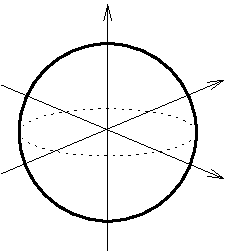
\includegraphics[width=39\unitlength]{sphere_lim}}
\cell{46}{20}{c}{x}
\cell{48}{36}{c}{y}
\cell{31}{51}{c}{z}
\cell{30}{4}{b}{\text{(a)}}
\end{picture}
% 
\hspace*{15mm}
% 
\setlength{\unitlength}{1mm}
\begin{picture}(34,48)(13,4)
\cell{30}{14.5}{b}{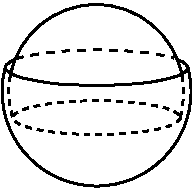
\includegraphics[width=33\unitlength]{sphere_colim}}
\cell{17}{43}{c}{D}
\cell{17}{17}{c}{D}
\cell{30}{4}{b}{\text{(b)}}
\end{picture}
\caption{Sphere as~(a) a limit, and~(b) a colimit.}
\label{fig:lim-colim-spheres}
\end{figure}

There is a kind of duality%
%
\index{duality}%
\index{limit!colimit@vs.\ colimit}
%
between the formulas for limits in $\Set$ (Example~\ref{eg:lims-Set}) and
colimits in $\Set$.  Whereas the limit is constructed as a \emph{subset} of
a \emph{product}, the colimit is a \emph{quotient}%
%
\index{quotient}
%
of a \emph{sum}.

Figure~\ref{fig:lim-colim-spheres} is intended to convey the difference in
flavour between limits and colimits, in a particular topological context.
In elementary texts, surfaces%
%
\index{surface|(}
%
are almost always seen as subsets of Euclidean space $\reals^3$, with the
sphere%
%
\index{sphere|(}
%
$S^2$ typically defined as
\[
\bigl\{ (x, y, z) \in \reals^3 \such x^2 + y^2 + z^2 = 1 \bigr\}.
\]
This is a \emph{subspace} of the \emph{product} space $\reals^3 = \reals
\times \reals \times \reals$, which suggests that it is a limit.  Indeed,
the sphere is the equalizer
\[
\xymatrix@M+.5ex{
S^2 \ar@{^{(}->}[r] &\reals^3 \ar@<.5ex>[r]^s \ar@<-.5ex>[r]_t&\reals
}
\]
where the maps $s, t \from \reals^3 \to \reals$ are given by
\[
s(x, y, z) = x^2 + y^2 + z^2,
\qquad
t(x, y, z) = 1.
\]
(An \emph{equa}tion is captured by an \emph{equa}lizer.)%
%
\index{equalizer}
%
  
In more advanced mathematics, however, this point of view is used less
often.  A surface can instead be thought of as the gluing-together of lots
of little patches, each isomorphic to the open unit disk $D$.  For example,
we could in principle construct an entire bicycle%
%
\index{bicycle inner tube}
%
inner tube by gluing together a large number of puncture-repair patches.
Figure~\ref{fig:lim-colim-spheres}(b) shows the simpler example of a sphere
made up of two disks glued together.  This realizes the sphere as a
\emph{quotient} (gluing) of the \emph{sum} (disjoint union) of the two
copies of $D$, suggesting that we have constructed the sphere as a colimit.
Indeed, the sphere is the coequalizer
\[
\xymatrix@M+.5ex{
S^1 \times (0, 1) \ar@<.7ex>@{^{(}->}[r] \ar@<-.7ex>@{^{(}->}[r]      &
D + D \ar[r] &S^2
}
\]
where $S^1$ is the circle, the cylinder $S^1 \times (0, 1)$ is the
intersection of the two copies of $D$ (the central belt of
Figure~\ref{fig:lim-colim-spheres}(b)), and the two maps into $D + D$ are
the inclusions of the cylinder into the first and second copies of $D$.%
%
\index{sphere|)}%
\index{surface|)}
%

One disadvantage of the limit point of view is that it makes an arbitrary
choice of coordinate system.  It is generally best to think of spaces as
free-standing objects, existing independently of any particular embedding into
Euclidean space.  

One disadvantage of the colimit point of view is that it makes an arbitrary
choice of decomposition.  For example, we could decompose the sphere into
three patches rather than two, or use a different two patches from those
shown.

The colimit point of view has the upper hand in modern geometry.  (If you
are familiar with the definition of manifold,%
%
\index{manifold}
%
you will recognize that an atlas is essentially a way of viewing a manifold
as a colimit of Euclidean balls.)  One reason for this is that we are often
concerned with maps \emph{out} of spaces $X$, such as maps $X \to \reals$.
Maps \emph{out} of a colimit are easy; it is in the very definition of
colimit that we know what the maps out of it are.


\minihead{Epics}


\begin{defn}
Let $\cat{A}$ be a category.  A map $X \toby{f} Y$ in $\cat{A}$ is
\demph{epic}%
%
\index{epic}
%
(or an \demph{epimorphism})%
%
\index{epimorphism}
%
if for all objects $Z$ and maps $\parpairi{Y}{Z}{g}{g'}$,
\[
g \of f = g' \of f
\implies 
g = g'.
\]
\end{defn}

This is the formal dual of the definition of monic.  (In other words, an
epic in $\cat{A}$ is a monic in $\cat{A}^\op$.)  It is in some sense the
categorical version of surjectivity.  But whereas the definition of monic
closely resembles the definition of injective, the definition of epic does
not look much like the definition of surjective.%
%
\index{function!surjective}%
\index{surjection}
%
The following examples confirm that in categories where surjectivity makes
sense, it is only sometimes equivalent to being epic.

\begin{example}        
In $\Set$, a map is epic%
%
\index{set!category of sets!epics in}
%
if and only if it is surjective.  If $f$ is surjective then certainly $f$
is epic.  To see the converse, take $Z$ to be a two-element set $\{ \true,
\false \}$, take $g$ to be the characteristic function of the image of $f$
(as defined in Section~\ref{sec:Set-properties}), and take $g'$ to be the
function with constant value $\true$.

Any isomorphism in any category is both monic and epic.  In $\Set$, the
converse also holds, since any injective surjective function is invertible
(Example~\ref{eg:iso-Set}). 
\end{example}

\begin{example}
\label{eg:epic-alg}
In categories of algebras, any surjective map is certainly epic.  In some
such categories, including $\Ab$, $\Vect_k$%
%
\index{vector space!category of vector spaces!epics in}
%
and $\Grp$,%
%
\index{group!category of groups!epics in}
%
the converse also holds.  (The proof is straightforward for $\Ab$ and
$\Vect_k$, but much harder for $\Grp$.)  However, there are other
categories of algebras where it fails.  For instance, in $\Ring$,%
%
\index{ring!category of rings!epics in}
%
the inclusion $\integers \incl \rationals$ is epic but not surjective
(Exercise~\ref{ex:epic-Ring}).  This is also an example of a map that is
monic and epic but not an isomorphism.
\end{example}

\begin{example}
In the category of Hausdorff topological spaces%
%
\index{topological space!category of topological spaces!epics in}%
\index{topological space!Hausdorff}
%
and continuous maps, any map with dense image is epic.
\end{example}

Of course, there is a dual of Lemma~\ref{lemma:monic-pb}, saying that a map is
epic if and only if a certain square is a pushout.


\exs


\begin{question}
Let $\parpair{X}{Y}{s}{t}$ be maps in some category.  Prove that $s = t$ if
and only if the equalizer of $s$ and $t$ exists and is an isomorphism, if
and only if the coequalizer of $s$ and $t$ exists and is an isomorphism.
\end{question}


\begin{question}
\begin{enumerate}[(b)]
\item 
Let $X$ be a set and $f\from X \to X$ a map.  Describe the coequalizer of
$\parpairi{X}{X}{f}{1}$ in $\Set$ as explicitly as possible. 

\item
Do the same in $\Tp$ rather than $\Set$.  When $X$ is the circle $S^1$,
find an $f$ such that the coequalizer is an uncountable space with the
indiscrete topology.
\end{enumerate}
\end{question}


\begin{question}        
\label{ex:epic-Ring}
\begin{enumerate}[(b)]
\item 
Prove that in the category of monoids,%
%
\index{monoid!epics between monoids}
%
the inclusion $(\nat, +, 0) \incl (\integers, +, 0)$ is epic, even though
it is not surjective.

\item 
Prove that in the category of rings, the inclusion $\integers \incl
\rationals$ is epic, even though it is not surjective.
\end{enumerate}
\end{question}


\begin{question}        
\label{ex:qt-objects}
(Compare Exercise~\ref{ex:subobjects}.)  Let $\cat{A}$ be a category and $A
\in \cat{A}$.  Define a \demph{quotient% 
%
\index{quotient}
%
object} of $A$ to be an isomorphism class of epics out of $A$.  That is,
let $\fcat{Epic}(A)$ be the full subcategory of $A/\cat{A}$ whose objects
are the epics; then a quotient object of $A$ is an isomorphism class of
objects of $\fcat{Epic}(A)$.
% 
\begin{enumerate}[(b)]
\item  
Let $A \toby{e} X$ and $A \toby{e'} X'$ be epics in $\Set$.  Show that $e$
and $e'$ are isomorphic in $\fcat{Epic}(A)$ if and only if they induce the
same equivalence%
%
\index{equivalence relation}
%
relation on $A$.  Deduce that the quotient objects of $A$ are in canonical
one-to-one correspondence with the equivalence relations on $A$.

\item 
Assuming the (nontrivial) fact that the epics in $\Grp$ are the
surjections, show that the quotient objects of a group correspond
one-to-one with its normal%
%
\index{group!normal subgroup of}
%
subgroups.
\end{enumerate}
% 
(The name `quotient object' is not standard, and indeed there is no
standard name for it.  Arguably, `quotient object' would be more suitable
for an isomorphism class of \emph{regular} epics, as defined in the
following exercises.)
\end{question}


\begin{question}        
\label{ex:reg-split-monic}
A map $m\from A \to B$ is \demph{regular%
%
\index{monic!regular}
%
monic} if there exist an object $C$ and maps $B \parpairu C$ of which $m$
is an equalizer.  A map $m\from A \to B$ is \demph{split%
%
\index{monic!split}
%
monic} if there exists a map $e\from B \to A$ such that $em = 1_A$.
% 
\begin{enumerate}[(b)]
\item 
Show that split monic $\implies$ regular monic $\implies$ monic.

\item 
In $\Ab$, show that all monics are regular but not all monics are split.
(Hint for the first part: equalizers in $\Ab$ are calculated as in
Example~\ref{eg:eq-vect}.)

\item 
In $\Tp$, describe the regular monics, and find a monic that is not
regular.  
\end{enumerate}
\end{question}


\begin{question}
Dualizing the definitions in Exercise~\ref{ex:reg-split-monic} gives
definitions of \demph{regular}%
%
\index{epic!regular}
%
and \demph{split%
%
\index{epic!split}
%
epic}.
% 
\begin{enumerate}[(b)]
\item 
We saw in Example~\ref{eg:epic-alg} that a map may be monic and epic but
not an isomorphism.  Prove that in any category, a map is an isomorphism if
and only if it is both monic and \emph{regular} epic.

\item 
Using the assumption that our category of sets satisfies the axiom of
choice (Section~\ref{sec:Set-properties}), show that
\[
\text{epic} \iff \text{regular epic} \iff \text{split epic}
\]
in $\Set$.

\item 
Let us say that a category $\cat{A}$ satisfies the \demph{axiom%
%
\index{axiom of choice}
%
of choice} if all epics in $\cat{A}$ are split.  Prove that neither $\Tp$
nor $\Grp$ satisfies the axiom of choice.
\end{enumerate}
\end{question}


\begin{question}
The result of Exercise~\ref{ex:pb-monic} can be phrased as `the class of
monics%
%
\index{monic!pullback of}%
\index{pullback!monic@of monic}
%
is stable under pullback'.  It is also a fact that the composite%
%
\index{monic!composition of monics}
%
of two monics is always monic; we say that the class of monics is `closed
under composition'.

Consider the following six classes of map:
% 
\begin{displaytext}
monics, regular monics, split monics,
epics, regular epics, split epics.
\end{displaytext}
% 
Determine whether each class is stable under pullback or closed under
composition.
\end{question}



\section{Interactions between functors and limits}
\label{sec:lims-ftrs}


We saw in Example~\ref{eg:lims-alg} that limits in categories such as
$\Grp$, $\Ring$ and $\Vect_k$ can be computed by first taking the limit in
the category of sets, then equipping the result with a suitable algebraic
structure.  On the other hand, colimits in these categories are unlike
colimits in $\Set$.  For example, the underlying set of the initial object
of $\Grp$ (which has one element) is not the initial object of $\Set$
(which has no elements), and the underlying set of the direct sum $X \oplus
Y$ of two vector spaces is not the sum of the underlying sets of $X$ and
$Y$.  So, these forgetful functors interact well with limits and badly with
colimits.

In this section, we develop terminology that will enable us to express
these thoughts precisely.

\begin{defn}
\begin{enumerate}[(b)]
\item   
\label{defn:pres-lims-shape}
Let $\scat{I}$ be a small category.  A functor $F\from \cat{A} \to \cat{B}$
\demph{preserves%
%
\index{limit!preservation of}
%
limits of shape $\scat{I}$} if for all diagrams $D\from \scat{I} \to
\cat{A}$ and all cones $\Bigl(A \toby{p_I} D(I)\Bigr)_{I \in \scat{I}}$ on
$D$,
% 
\begin{align*}
        &
\Bigl(A \toby{p_I} D(I)\Bigr)_{I \in \scat{I}}
\text{ is a limit cone on } D \text{ in }\cat{A}\\
\implies        &
\Bigl(F(A) \toby{Fp_I} FD(I)\Bigr)_{I \in \scat{I}}
\text{ is a limit cone on } F \of D \text{ in }\cat{B}. 
\end{align*}

\item   
\label{defn:pres-lims-all}
A functor $F\from \cat{A} \to \cat{B}$ \demph{preserves limits} if it
preserves limits of shape $\scat{I}$ for all small categories $\scat{I}$.

\item 
\demph{Reflection}%
%
\index{limit!reflection of}%
\index{reflection of limits}
%
of limits is defined as in~\bref{defn:pres-lims-shape}, but with $\textif$
in place of $\textonlyif$.
\end{enumerate}
\end{defn}
% 
Of course, the same terminology applies to colimits.

Here is a different way to state the definition of preservation.  A functor
$F\from \cat{A} \to \cat{B}$ preserves limits if and only if it has the
following property: whenever $D\from \scat{I} \to \cat{A}$ is a diagram
that has a limit, the composite $F \of D \from \scat{I} \to \cat{B}$ also
has a limit, and the canonical map
\[
F \biggl( \lt{\scat{I}} D \biggr)
\to
\lt{\scat{I}}(F \of D)
\]
is an isomorphism.  Here the `canonical map' has $I$-component 
\[
F \biggl( \lt{\scat{I}} D \biggr)
\toby{F(p_I)}
F(D(I)),
\]
where $p_I$ is the $I$th projection of the limit cone on $D$.

In particular, if $F$ preserves limits then
% 
\begin{equation}
\label{eq:lim-pres-rough}
F \biggl( \lt{\scat{I}} D \biggr)
\iso
\lt{\scat{I}}(F \of D)
\end{equation}
% 
whenever $D$ is a diagram with a limit.  Preservation of limits says more
than \eqref{eq:lim-pres-rough} does: the left- and right-hand sides are
required to be not just isomorphic, but isomorphic \emph{in a particular
  way}.  Nevertheless, we will sometimes omit this check, acting as if
preservation means only that~\eqref{eq:lim-pres-rough} holds.

\begin{example}
The forgetful functor $U\from \Tp \to \Set$%
%
\index{topological space!category of topological spaces!limits in}%
\index{topological space!category of topological spaces!colimits in}
%
preserves both limits and colimits.  (As we will see, this follows from the
fact that $U$ has adjoints on both sides.)  It does not reflect all limits
or all colimits.  For instance, choose any non-discrete spaces $X$ and $Y$,
and let $Z$ be the set $U(X) \times U(Y)$ equipped with the discrete
topology.  (All that matters here is that the topology on $Z$ is strictly
larger than the product topology.)  Then we have a cone
% 
\begin{equation}        
\label{eq:discrete-pjn}
X \ot Z \to Y
\end{equation}
% 
in $\Tp$ whose image in $\Set$ is the product cone
\[
U(X) \ot U(X) \times U(Y) \to U(Y).
\]
But~\eqref{eq:discrete-pjn} is not a product cone in $\Tp$, since the
discrete topology on $U(X) \times U(Y)$ is not the product topology.
\end{example}

\begin{example}
In the first paragraph of this section, we observed that the forgetful
functor $\Grp \to \Set$%
%
\index{group!category of groups!colimits in}
%
does not preserve initial objects and that the forgetful functor $\Vect_k
\to \Set$%
%
\index{vector space!category of vector spaces!colimits in}
%
does not preserve binary sums.  Forgetful functors out of categories of
algebras very seldom preserve all colimits.
\end{example}

\begin{example} 
\label{eg:gp-creation}
%
\index{group!category of groups!limits in|(}%
\index{vector space!category of vector spaces!limits in|(}%
\index{ring!category of rings!limits in|(}
%
We also saw that (in the examples mentioned) forgetful functors on
categories of algebras do preserve limits.  In fact, something stronger is
true.  Let us examine the case of binary products in $\Grp$, although all
of the following can be said for any limits in any of the categories
$\Grp$, $\Ab$, $\Vect_k$, $\Ring$, etc.

Take groups $X_1$ and $X_2$.  We can form the product set $U(X_1) \times
U(X_2)$, which comes equipped with projections
\[
U(X_1) \otby{p_1} U(X_1) \times U(X_2) \toby{p_2} U(X_2).
\]
I claim that there is exactly one group structure on the set $U(X_1) \times
U(X_2)$ with the property that $p_1$ and $p_2$ are homomorphisms.  To prove
uniqueness, suppose that we have a group structure on $U(X_1) \times U(X_2)$
with this property.  Take elements $(x_1, x_2)$ and $(x'_1, x'_2)$ of
$U(X_1) \times U(X_2)$ and write $(x_1, x_2) \cdot (x'_1, x'_2) = (y_1,
y_2)$.  Since $p_1$ is a homomorphism,
\[
y_1
=
p_1(y_1, y_2)
=
p_1((x_1, x_2) \cdot (x'_1, x'_2))
=
p_1(x_1, x_2) \cdot p_1(x'_1, x'_2)
=
x_1 \cdot x'_1,
\]
and similarly $y_2 = x_2 \cdot x'_2$.  Hence 
\[
(x_1, x_2) \cdot (x'_1, x'_2) = (x_1 x'_1, x_2 x'_2).  
\]
A similar argument shows that $(x_1, x_2)^{-1} = (x_1^{-1}, x_2^{-1})$ and
that the identity element $1$ of the group is $(1, 1)$.  Now, for
existence, define $\cdot$, $\blank^{-1}$ and $1$ by the formulas just
given; it can then be checked that the group axioms are satisfied and that
$p_1$ and $p_2$ are group homomorphisms.  This proves the claim.

Write $L$ for the set $U(X_1) \times U(X_2)$ equipped with this group
structure.  Then we have a cone
\[
X_1 \otby{p_1} L \toby{p_2} X_2
\]
in $\Grp$.  It is easy to check that this is, in fact, a \emph{product}
cone in $\Grp$.

We can summarize this in language that is not tied to group theory.  Given
objects $X_1$ and $X_2$ of $\Grp$,
% 
\begin{itemize}
\item 
for any product cone on $(U(X_1), U(X_2))$ in $\Set$, there is a unique
cone on $(X_1, X_2)$ in $\Grp$ whose image under $U$ is the cone we started
with; 

\item 
this cone on $(X_1, X_2)$ is a product cone.
\end{itemize}
\end{example}
% 
This suggests the following definition (Figure~\ref{fig:creation}).

\begin{figure}
\centering
\setlength{\unitlength}{1em}
\begin{picture}(12.8,14)(-5.6,-7)
\cell{0}{0}{c}{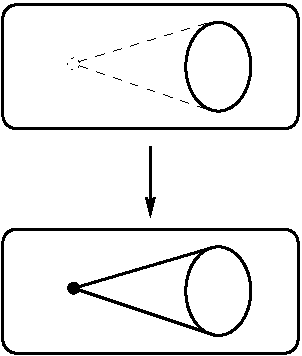
\includegraphics[height=14\unitlength]{creation}}
\cell{6.7}{4.4}{c}{\cat{A}}
\cell{2.7}{4.4}{c}{D}
\cell{-0.2}{4.3}{c}{p}
\cell{-3.8}{4.4}{c}{A}
\cell{1}{0}{c}{F}
\cell{6.7}{-4.4}{c}{\cat{B}}
\cell{2.7}{-4.4}{c}{F \!\of\! D}
\cell{-0.2}{-4.5}{c}{q}
\cell{-3.8}{-4.4}{c}{B}
\end{picture}%
\caption{Creation of limits.}
\label{fig:creation}
\end{figure}

\begin{defn}    
\label{defn:creates}
A functor $F\from \cat{A} \to \cat{B}$ \demph{creates%
%
\index{limit!creation of|(}%
\index{creation of limits|(}
%
limits (of shape $\scat{I}$)} if whenever $D\from \scat{I} \to \cat{A}$ is
a diagram in $\cat{A}$,
% 
\begin{itemize}
\item 
for any limit cone $\Bigl(B \toby{q_I} FD(I)\Bigr)_{I \in \scat{I}}$ on
the diagram $F \of D$, there is a unique cone $\Bigl(A \toby{p_I}
D(I)\Bigr)_{I \in \scat{I}}$ on $D$ such that $F(A) = B$ and $F(p_I) = q_I$
for all $I \in \scat{I}$;

\item 
this cone $\Bigl(A \toby{p_I} D(I)\Bigr)_{I \in \scat{I}}$ is a limit cone
on $D$.
\end{itemize}
\end{defn}
% 
The forgetful functors from $\Grp$, $\Ring$, \ldots\ to $\Set$ all create
limits (Exercise~\ref{ex:fgt-create}).  The word \emph{creates} is
explained by the following result.

\begin{lemma}   
\label{lemma:creates-preserves}
Let $F \from \cat{A} \to \cat{B}$ be a functor and $\scat{I}$ a small
category.  Suppose that $\cat{B}$ has, and $F$ creates, limits of shape
$\scat{I}$.  Then $\cat{A}$ has, and $F$ preserves, limits of shape
$\scat{I}$. 
\end{lemma}

\begin{pf}
Exercise~\ref{ex:creates-preserves}.
\end{pf}

Since $\Set$ has all limits, it follows that all our categories of algebras
have all limits, and that the forgetful functors preserve them.

\begin{remark}
There is something suspicious about Definition~\ref{defn:creates}.  It
refers to \emph{equality} of objects of a category, a relation that, as we
saw on page~\pageref{p:care}, is usually too strict to be appropriate.  It
is almost always better to replace equality by isomorphism.  If we replace
equality by isomorphism throughout the definition of `creates limits', we
obtain a more healthy and inclusive notion.  In the notation of
Definition~\ref{defn:creates}, we ask that if $F \of D$ has a limit then
there exists a cone on $D$ whose image under $F$ is a limit cone, and that
every such cone is itself a limit cone.  

In fact, what we are calling creation of limits should really be called
\emph{strict} creation of limits, with `creation of limits' reserved for
the more inclusive notion.  That is how `creates' is used in most of the
literature.  I have chosen to use the strict version here because it is
slightly simpler to state, and because the examples at hand all satisfy the
stricter condition.
%
\index{limit!creation of|)}%
\index{creation of limits|)}%
\index{group!category of groups!limits in|)}%
\index{vector space!category of vector spaces!limits in|)}%
\index{ring!category of rings!limits in|)}
%
\end{remark}


\exs


\begin{question}        
\label{ex:prod-Set-functorial}
Taking the limit is a process that receives as its input a diagram in a
category $\cat{A}$, and produces as its output a new object of $\cat{A}$.
Later, we will see that this process is functorial%
%
\index{limit!functoriality of}
%
(Proposition~\ref{propn:lim-const-adjn}).  Here you are asked to prove this
in the case of binary products.%
%
\index{product!functoriality of}
%

Let $\cat{A}$ be a category with binary products.  Suppose that we have chosen
for each pair $(X, Y)$ of objects a product cone
\[
\xymatrix@1{
X       &X \times Y \ar[l]_{p^{X, Y}_1} \ar[r]^-{p^{X, Y}_2}     &Y.
}
\]
Construct a functor $\cat{A} \times \cat{A} \to \cat{A}$ given on objects
by $(X, Y) \mapsto X \times Y$.
\end{question}


\begin{question}
Let $\cat{A}$ be a category with binary products.  Prove directly that 
\[
\cat{A}(A, X \times Y)
\iso 
\cat{A}(A, X) \times \cat{A}(A, Y)
\]
naturally in $A, X, Y \in \cat{A}$.  (This presupposes that we have chosen
for each $X$ and $Y$ a product cone on $(X, Y)$.  By
Exercise~\ref{ex:prod-Set-functorial}, the assignment $(X, Y) \mapsto X
\times Y$ is then functorial, which it must be in order for `naturally' to
make sense.)
\end{question}


\begin{question}
Prove that if a functor creates limits then it also reflects them. 
\end{question}


\begin{question}        
\label{ex:fgt-create}
It was shown in Example~\ref{eg:gp-creation} that the forgetful functor
$U\from \Grp \to \Set$%
%
\index{group!category of groups!limits in}
%
creates binary products.
% 
\begin{enumerate}[(b)]
\item
Using the formula for limits in $\Set$ (Example~\ref{eg:lims-Set}), prove
that, in fact, $U$ creates arbitrary limits.

\item
Satisfy yourself that the same is true if $\Grp$ is replaced by any other
category of algebras such as $\Ring$,%
%
\index{ring!category of rings!limits in}
%
$\Ab$ or $\Vect_k$.%
%
\index{vector space!category of vector spaces!limits in}
%
\end{enumerate}
\end{question}


\begin{question}        
\label{ex:creates-preserves}
Prove Lemma~\ref{lemma:creates-preserves}.
\end{question}


\begin{question}
\begin{enumerate}[(b)]
\item 
An object $P$ of a category $\cat{B}$ is \demph{projective}%
%
\index{projective object}%
\index{object!projective}
%
if $\cat{B}(P, \dashbk) \from \cat{B} \to \Set$ preserves epics.  (This
means that if $f$ is epic then so is $\cat{B}(P, f)$.)  Let
$\hadjnli{\Set}{\cat{B}}{F}{G}$ be an adjunction in which $G$ preserves
epics.  Prove that $F(S)$ is projective for all sets $S$.

\item 
Find a non-projective object of $\Ab$.

\item 
An object $I$ of a category $\cat{B}$ is \demph{injective}%
%
\index{injective object}%
\index{object!injective}
%
if it is projective in $\cat{B}^\op$, or equivalently if $\cat{B}(\dashbk,
I)\from \cat{B}^\op \to \Set$ preserves epics.  Show that all objects of
$\Vect_k$ are injective, and find a non-injective object of $\Ab$.
\end{enumerate}
\end{question}



